\documentclass[12pt,a4paper]{article}
\usepackage[UTF8]{ctex}
\usepackage{geometry}
\usepackage{amsmath,amssymb,amsthm}
\usepackage{mathtools,bm}
\usepackage{empheq}
\usepackage{graphicx}
\usepackage{booktabs}
\usepackage[numbers,sort&compress]{natbib}
\usepackage{caption}
\usepackage{enumitem}
\usepackage{chngcntr}
\usepackage{tikz}

% ========== 页面布局 ==========
\geometry{left=2.5cm,right=2.5cm,top=2.5cm,bottom=2.5cm}
\setlength{\parskip}{0.5em}
\renewcommand{\baselinestretch}{1.2}

% ========== 数学命令 ==========
\newcommand{\diff}{\mathop{}\!\mathrm{d}}
\newcommand{\R}{\mathbb{R}}
\newcommand{\C}{\mathbb{C}}
\newcommand{\Z}{\mathbb{Z}}
\newcommand{\N}{\mathbb{N}}
\DeclareMathOperator{\supp}{supp}

% ========== 编号系统 ==========
\numberwithin{subsection}{section}   % 子小节按章节编号
\numberwithin{subsubsection}{subsection}
\counterwithin{equation}{subsection} % 公式按子小节编号

% ========== 定理环境 ==========
\theoremstyle{plain}
\newtheorem{theorem}{定理}[section]
\newtheorem{lemma}[theorem]{引理}
\newtheorem{proposition}[theorem]{命题}
\newtheorem{corollary}[theorem]{推论}
\newtheorem{solution}{解}[subsection]  % 解按子小节编号

\theoremstyle{definition}
\newtheorem{definition}[theorem]{定义}
\newtheorem{example}{例题}[subsection]  % 示例按子小节编号

\theoremstyle{remark}
\newtheorem{remark}[theorem]{注记}

\theoremstyle{remark}
\newtheorem{verification}[theorem]{验证}

% 加载hyperref包以实现超链接功能
\usepackage[colorlinks=true, linkcolor=black]{hyperref}

\title{偏微分方程笔记}
\author{陈柏均}
\date{2025年5月12日}

\begin{document}
	
	\maketitle

 \begin{abstract}
	 首先,对于一般的有界偏微分方程,如果三个条件都是线性的就可以用叠加原理分解为三个子问题;同理无界的时候,如果也是线性的,就可以分解成两个子问题。
	 
	 对于边界条件非齐次,我们运用数值分析中,插值拟合函数的思想来齐次化,有很多插值的方法,这里我们选择多项式插值,而且为简化后面的计算,让多项式的次数尽量最低。
	 
	 对于方程非齐次,就用duhamel原理齐次化方程。不管是有界,什么类型的边界条件,还是无界,都可以用他,把函数转移到初始条件最高阶偏导函数上,再积分就是方程的解。
	 
	 对于无界齐次的波动方程,用达朗贝尔公式。要解达朗贝尔公式要先解传输方程。5.1,5.2用不同的思路求解齐次的传输方程。由达朗贝尔公式可知,变量替换后两变量不会杂糅。由达朗贝尔公式可得依赖区域,影响区域,决定区域和特征线的关系。
	 
	 对于无界齐次的热传导方程,用泊松公式。泊松公式的推导需要卷积,傅里叶变换的一些知识。用傅里叶变换不用自相似变换是因为我觉得傅里叶变换更直接明了。
	 
	 对于各种有界的情况,不管是波动还是热传导都可以用分离变量法,他是一种思路,并不是像达朗贝尔公式和泊松公式只针对一类方程的通解。根据不同的边界条件做变化,得不同的解,但是它们思路都是一样,就是得通解之后,根据不同的边界条件来待定系数。
	 
	 对于有界的波动还是热传导,我们还可以用无界解达朗贝尔公式和泊松公式做一些特殊的延拓来求解。对于第一边界条件我们先奇延拓再周期延拓;对于第二边界条件我们先偶延拓再周期延拓。但是必须满足一定的相容性条件。所以对于有界的还是分离变量法能求解任何情况,这个更稳妥。
	 
	 对于半直线的波动还是热传导问题,就是用无界解达朗贝尔公式和泊松公式做延拓,第一边界条件做奇延拓,第二边界条件做偶延拓。
\end{abstract}


\newpage
	
	\tableofcontents  % 添加目录
	
	
	\newpage
	\section{按边界条件分类偏微分方程}
	一般的偏微分方程是由空间变量$x \in \R$和时间变量$t \geq 0$构成的问题,有三个条件:方程,初始条件($t=0$),边界条件($x=0, \quad l=0$).
	  
	  根据空间变量$x$的范围,即边界条件可以分类成三类问题,再根据每类问题的边界条件是原函数还是一阶导函数可分类子问题7个。
	  
	  下面用波动方程举例,方程原则上可以算任意方程。
	\subsection{有界}
	有界指的是空间变量$x \in [0,l]$和时间变量$t \geq 0$.
	
	$x=0,\quad l=0$都有函数,可能都是原函数(第一类边界,也叫Dirichlet边界条件);可能都是一阶导函数(第二类边界);可能一个是原函数,另一个是一阶偏导函数(混合边界,有两个)。
	\subsubsection{第一类边界}
	$x=0,\quad l=0$都是原函数。
	\begin{equation}\label{The bounded wave equation with Dirichlet boundary conditions}
		\begin{cases}
			u_{tt} - a^2 u_{xx} = f(x, t), & 0 < x < l, \ t > 0, \\
			u(x, 0) = \varphi(x), \ u_t(x, 0) = \psi(x), & 0 \leq x \leq l, \\
			u(0, t) = \mu_1(t), \ u(l, t) = \mu_2(t), & t \geq 0.
		\end{cases}
	\end{equation}
		\subsubsection{第二类边界}
			$x=0,\quad l=0$都是一阶偏导函数。
		\begin{equation}\label{The bounded wave equation with Neumann boundary conditions}
			\begin{cases}
				u_{tt} - a^2 u_{xx} = f(x, t), & 0 < x < l, \ t > 0, \\
				u(x, 0) = \varphi(x), \ u_t(x, 0) = \psi(x), & 0 \leq x \leq l, \\
            	u_x(0, t) = \mu_1(t), \ u_x(l, t) = \mu_2(t), & t \geq 0.
			\end{cases}
		\end{equation}
		
		
		\subsubsection{两种混合}
	第一种:$x=0$处是原函数,$ l=0$是一阶偏导函数。
		\begin{equation}\label{The bounded wave equation with mixed boundary conditions_1}
			\begin{cases}
				u_{tt} - a^2 u_{xx} = f(x, t), & 0 < x < l, \ t > 0, \\
				u(x, 0) = \varphi(x), \ u_t(x, 0) = \psi(x), & 0 \leq x \leq l, \\
				u(0, t) = \mu_1(t), \ u_x(l, t) = \mu_2(t), & t \geq 0.
			\end{cases}
			\end{equation}
		
			第二种:$x=0$处是一阶偏导函数,$ l=0$是原函数。
		\begin{equation}\label{The bounded wave equation with mixed boundary conditions_2}
			\begin{cases}
				u_{tt} - a^2 u_{xx} = f(x, t), & 0 < x < l, \ t > 0, \\
				u(x, 0) = \varphi(x), \ u_t(x, 0) = \psi(x), & 0 \leq x \leq l, \\
				u_x(0, t) = \mu_1(t), \ u(l, t) = \mu_2(t), & t \geq 0.
			\end{cases}
				\end{equation}
				
		
		
\subsection{半直线}
半直线指空间变量$x \geq 0$,时间变量$t \geq 0$

故边界条件只有$x=0$一个,再根据第一边界,第二边界就可以分成两类。
\subsubsection{第一边界}
\begin{equation}\label{The wave equation on a half-line with Dirichlet boundary conditions}
	\begin{cases}
		u_{tt} - a^2 u_{xx} = f(x, t), & x > 0, \ t > 0, \\
		u(x, 0) = \varphi(x), \ u_t(x, 0) = \psi(x), & x > 0, \\
     	u(0, t) = \mu_1(t), & t \geq 0.
	\end{cases}
	\end{equation}
	
\subsubsection{第二边界}
\begin{equation}\label{The wave equation on a half-line with Neumann boundary conditions}
	\begin{cases}
		u_{tt} - a^2 u_{xx} = f(x, t), &  x > 0, \ t > 0, \\
		u(x, 0) = \varphi(x), \ u_t(x, 0) = \psi(x), & x > 0, \\
		u_x(0, t) = \mu_1(t), & t \geq 0.
	\end{cases}
	\end{equation}

	\subsection{无界}
	
	\begin{equation}\label{The unbounded wave equation}
		\begin{cases}
			u_{tt} - a^2 u_{xx} = f(x, t), &  x \in (-\infty , +\infty), \ t > 0, \\
			u(x, 0) = \varphi(x), \ u_t(x, 0) = \psi(x), & x \in (-\infty , +\infty) \\
		\end{cases}
	\end{equation}
	
	
	
		\newpage
	\section{叠加原理}
	叠加原理是一种思想,和分离变量法一样。对于三个非齐次条件都是线性的,就可以分解成三个方程的叠加。下面举第一边界条件的有界波动方程做例子.
	
	对于问题\eqref{The bounded wave equation with Dirichlet boundary conditions},我们可以使用叠加原理将其分解为3个子问题.
		\subsection{方程非齐次}
				\begin{equation}\label{q1}
		\begin{cases}
			u_{tt} - a^2 u_{xx} = f(x, t), & 0 < x < l, \ t > 0, \\
			u(x, 0) = 0, \ u_t(x, 0) = 0, & 0 \leq x \leq l, \\
			u(0, t) = 0, \ u(l, t) = 0, & t \geq 0.
		\end{cases}
	\end{equation}
	\begin{remark}
	对于方程\eqref{q1}我们用Duhamamel原理,将方程齐次化,方程的函数转移到初始条件最高偏导函数上,与7个边界条件没有关系,化成方程\eqref{q2}.
	\end{remark}
		
	\subsection{初始条件非齐次}
		\begin{equation}\label{q2}
			\begin{cases}
				u_{tt} - a^2 u_{xx} = 0, & 0 < x < l, \ t > 0, \\
				u(x, 0) = \varphi(x), \ u_t(x, 0) = \psi(x), & 0 \leq x \leq l, \\
				u(0, t) = 0, \ u(l, t) = 0, & t \geq 0.
			\end{cases}
		\end{equation}
\begin{remark}
	这个也是最基础的方程,方程\eqref{q1}和\eqref{q3}都可以齐次化成这样的方程,故这个方程是我们最终要解决的方程。
\end{remark}
	
	
	\subsection{边界条件非齐次}
	\begin{equation}\label{q3}
		\begin{cases}
			u_{tt} - a^2 u_{xx} = 0, & 0 < x < l, \ t > 0, \\
			u(x, 0) = 0, \ u_t(x, 0) = 0, & 0 \leq x \leq l, \\
			u(0, t) = \mu_1(t), \ u(l, t) = \mu_2(t), & t \geq 0.
		\end{cases}
	\end{equation}	
	
	通过数值分析中的线性插值可以把任何边界条件其次化,转化成下面的方程:
	\begin{equation}\label{q3.1}
	\begin{cases}
		v_{tt} - a^2 v_{xx} = f_1(x, t), & 0 < x < l, \ t > 0, \\
		v|_{t=0} = \varphi_1(x), \quad v_t|_{t=0} = \psi_1(x), & 0 \leq x \leq l, \\
		v|_{x=0} = 0, \quad v|_{x=l} = 0, & t \geq 0.
	\end{cases}
\end{equation}
	
	
	\begin{remark}
	对于问题\eqref{q3.1},我们可以使用叠加原理将其分解为两个子问题,又回到上面的两个方程\eqref{q1}和\eqref{q2}
\end{remark}

	

	
	\newpage
	
		\section{边界条件齐次化}
		本质上就是数值分析上的插值。知道两个端点的信息或者一个点的信息,用函数拟合插值。我这里不需要拟合,原则上可以选取任意满足边界条件的函数,为了方便后面的方程计算,我们一般选取牛顿插值法,即多项式插值。	
		
		因为我们只有两个条件,但是如果是多次,比如四次的多项式有4个未知数,而这些未知数我们可以随便取,故我们一般为简化后面的计算,让待定的最高的系数为0(原则上我们取多少次多项式都可以,但是为了后面的计算我们肯定是想让次数最低)
		
		第一边界条件两个都是原函数,明显用一次,两个参数就可以被确定;第二边界条件两个都是导函数,明显用二次多项式,求导后为一次,两个参数可根据导函数确定;故混合边界条件一定不会超过二次。所以我们干脆混合边界条件直接全部取二次就好了,到时候让最高次待定系数为0就好(如果你看了后面,其实都是一次,我这里只是为了思路通畅)
	\subsection{第一边界条件齐次化}
	要想利用Duhamamel原理,我们首先将第一边界条件齐次化,即要找到一个恰当的变换将第一边界值变为零。
	对于第一类边界条件的有界波动方程\eqref{The bounded wave equation with Dirichlet boundary conditions}:
	
	由边界条件
	\begin{equation}
		u(0,t) = \mu_1(t), \quad u(l,t) = \mu_2(t), \quad t \geq 0.
	\end{equation}
	
	设$U(x, t)=ax+b$
	\[
	\begin{cases}
		u(0, t) = \mu_1(t) = U(0, t) = b, \\
		u(l, t) = \mu_2(t) = U(l, t) = al + \mu_1(t),
	\end{cases}
	\]
	\[
	\begin{cases}
		a = \frac{1}{l}(\mu_2(t) - \mu_1(t)), \\
		b = \mu_1(t).
	\end{cases}
	\]
	对方程 \eqref{The bounded wave equation with Dirichlet boundary conditions}构造关于变量 \(x\) 的线性辅助函数(直线方程):
	\begin{equation}
		U(x, t) = \mu_1(t) + \frac{x}{l}(\mu_2(t) - \mu_1(t)),
	\end{equation}
	
	作变换:
	\begin{equation}
		v(x, t) = u(x, t) - U(x, t),
	\end{equation}
	
	 代入方程\eqref{The bounded wave equation with Dirichlet boundary conditions},
	得到方程\eqref{A}:
	\begin{equation}\label{A}
	\begin{cases}
		v_{tt} - a^2 v_{xx} = f_1(x, t), & 0 < x < l, \ t > 0, \\
		v(x, 0) = \varphi_1(x), \quad v_t(x, 0) = \psi_1(x), & 0 \leq x \leq l, \\
		v(0, t) = 0, \quad v(l, t) = 0. &
	\end{cases}
\end{equation}
	其中:
	\begin{equation}
		\begin{cases}
			f_1(x, t) = f(x, t) - \mu_1''(t) - \frac{x}{l}(\mu_2''(t) - \mu_1''(t)), \\
			\varphi_1(x) = \varphi(x) - \mu_1(0) - \frac{x}{l}(\mu_2(0) - \mu_1(0)), \\
			\psi_1(x) = \psi(x) - \mu_1'(0) - \frac{x}{l}(\mu_2'(0) - \mu_1'(0)).
		\end{cases}
	\end{equation}
	
	这样我们就完成了第一边界条件的齐次化。
	
	\subsection{第二边界条件齐次化}
	为利用Duhamel原理,需将非齐次Neumann边界条件齐次化,即构造变换使边界导数归零。

		
		以下我们仅考虑如下第二边界条件的有界波动方程\eqref{The bounded wave equation with Neumann boundary conditions}:
		
		设$U(x, t)=ax^2+bx+c$
		\[
		\begin{cases}
			u_x(0, t) = \mu_1(t) = U_x(0, t) = b, \\
			u_x(l, t) = \mu_2(t) = U_x(l, t) = 2al + b,
		\end{cases}
		\]
		\[
		\begin{cases}
			a = \frac{1}{2l}(\mu_2(t) - \mu_1(t)) \\
			b = \mu_1(t) \\
			c = 0 
		\end{cases}
		\]
		
		构造辅助函数:
		\begin{equation}
			U(x, t) = x\mu_1(t) + \frac{x^2}{2l}\big( \mu_2(t) - \mu_1(t) \big),
		\end{equation}
		
		作变换:
		\begin{equation}
			v(x, t) = u(x, t) - U(x, t),
		\end{equation}
		
		代入原方程\eqref{The bounded wave equation with Neumann boundary conditions},
		得到方程\eqref{B}:
	    \begin{equation}\label{B}
		\begin{cases}
			v_{tt} - a^2 v_{xx} = f_2(x, t), & 0 < x < l, \ t > 0, \\
			v(x, 0) = \varphi_2(x), \quad v_t(x, 0) = \psi_2(x), & 0 \leq x \leq l, \\
			v_x(0, t) = 0, \quad v_x(l, t) = 0. &
		\end{cases}
	\end{equation}

其中:
		\begin{equation}
			\begin{cases}
				f_2(x, t) = f(x, t)-x\mu_1''(t) - \frac{x^2}{2l}\big( \mu_2''(t) - \mu_1''(t) \big) + \frac{a^2}{l}\big( \mu_2(t) - \mu_1(t) \big), \\
				\varphi_2(x) = \varphi(x) - x\mu_1(0) - \frac{x^2}{2l}\big( \mu_2(0) - \mu_1(0) \big), \\
			\psi_2(x) = \psi(x) - x\mu_1'(0) - \frac{x^2}{2l}\big( \mu_2'(0) - \mu_1'(0) \big), 
			\end{cases}
		\end{equation}
		
	
		
	\subsection{第一混合边界条件齐次化}
	本质上就是数值分析上的插值,原理同上。
	对于问题\eqref{The bounded wave equation with mixed boundary conditions_1}
	
		由边界条件
	\begin{equation}
		u(0,t) = \mu_1(t), \quad u_x(l,t) = \mu_2(t), \quad t \geq 0.
	\end{equation}
	
	设$u(x, t)=U(x, t)=ax^2+bx+c$
	\[
	\begin{cases}
		u(0, t) = \mu_1(t) = U(0, t) = c, \\
		u_x(l, t) = \mu_2(t) = U_x(l, t) = 2al + b,
	\end{cases}
	\]
	\[
	\begin{cases}
		a = 0 (\text{令最高次待定系数为0})\\
		b =\mu_2(t) \\
		c = \mu_1(t)
	\end{cases}
	\]
	
	对方程 \eqref{The bounded wave equation with mixed boundary conditions_1}构造关于变量 \(x\) 的线性辅助函数(直线方程):
	\begin{equation}
		U(x, t) =  \mu_2(t) x+\mu_1(t) ,
	\end{equation}
	
	作变换:
	\begin{equation}
		v(x, t) = u(x, t) - U(x, t),
	\end{equation}
	
	代入方程\eqref{The bounded wave equation with mixed boundary conditions_1},
	得到方程\eqref{C}:
	\begin{equation}\label{C}
		\begin{cases}
			v_{tt} - a^2 v_{xx} = f_3(x, t), & 0 < x < l, \ t > 0, \\
			v(x, 0) = \varphi_3(x), \quad v_t(x, 0) = \psi_3(x), & 0 \leq x \leq l, \\
			v(0, t) = 0, \quad v_x(l, t) = 0. &
		\end{cases}
	\end{equation}
	其中:
\begin{equation}
	\begin{cases}
		f_3(x, t) = f(x, t) - (\mu_2''(t)x + \mu_1''(t)), \\
		\varphi_3(x) = \varphi(x) - (\mu_2(0)x + \mu_1(0)), \\
		\psi_3(x) = \psi(x) - (\mu_2'(0)x + \mu_1'(0)).
	\end{cases}
\end{equation}
	
	
		\subsection{第二混合边界条件齐次化}
	本质上就是数值分析上的插值,原理同上。
	对于问题\eqref{The bounded wave equation with mixed boundary conditions_2}
	
	由边界条件
	\begin{equation}
		u_x(0,t) = \mu_1(t), \quad u(l,t) = \mu_2(t), \quad t \geq 0.
	\end{equation}
	
	设$u(x, t)=U(x, t)=ax^2+bx+c$
	\[
	\begin{cases}
		u_x(0, t) = \mu_1(t) = U_x(0, t) = b, \\
		u(l, t) = \mu_2(t) = U(l, t) = al^2 + bl+c,
	\end{cases}
	\]
	\[
	\begin{cases}
		a = 0 (\text{令最高次待定系数为0})\\
	b =\mu_1(t) \\
	c = \mu_2(t)-\mu_1(t)l
	\end{cases}
	\]
	
	对方程 \eqref{The bounded wave equation with mixed boundary conditions_2}构造关于变量 \(x\) 的线性辅助函数(直线方程):
	\begin{equation}
		U(x, t) = \mu_1(t)(x-l) + \mu_2(t) ,
	\end{equation}
	
	作变换:
	\begin{equation}
		v(x, t) = u(x, t) - U(x, t),
	\end{equation}
	
	代入方程\eqref{The bounded wave equation with mixed boundary conditions_2},
	得到方程\eqref{D}:
	\begin{equation}\label{D}
		\begin{cases}
			v_{tt} - a^2 v_{xx} = f_4(x, t), & 0 < x < l, \ t > 0, \\
			v(x, 0) = \varphi_4(x), \quad v_t(x, 0) = \psi_4(x), & 0 \leq x \leq l, \\
			v_x(0, t) = 0, \quad v_x(l, t) = 0. &
		\end{cases}
	\end{equation}
	其中:
	\begin{equation}
		\begin{cases}
			f_4(x, t) = f(x, t) - \mu_1''(t) (x-l)- \mu_2''(t) , \\
			\varphi_4(x) = \varphi(x) - \mu_1(0)(x-l)- \mu_2(0), \\
			\psi_4(x) = \psi(x) - \mu_1'(0)(x-l) - \mu_2'(0).
		\end{cases}
	\end{equation}
	
	
	\subsection{总结}
	由上可得其实就是第二边界条件需要设二次多项式,其他都是一次就可以了。
	
	
	
		\newpage
	\section{Duhamamel原理之方程齐次化}
不管是第一边界条件,第二边界条件,混合边界条件,无界情况都一样。因为方程齐次化只与方程和初始条件有关,与边界边界条件无关。下面只举第一边界,无界的。
	
	
		\subsection{有界非齐次方程}

		
	对于第一边界非齐次方程问题:
	\begin{equation}
		\begin{cases}
			v_{tt} - a^2 v_{xx} = f_1(x, t), & 0 < x < l, \ t > 0, \\
			v|_{t=0} = 0, \quad v_t|_{t=0} = 0, & 0 \leq x \leq l, \\
			v|_{x=0} = 0, \quad v|_{x=l} = 0, & t \geq 0,
		\end{cases}
	\end{equation}
	
	若 \( W(x, t, \tau) \) 是以下定解问题的解:
\begin{equation}
	\begin{cases}
		W_{tt} - a^2 W_{xx} = 0, & 0 \leq x \leq l, t > \tau, \\
	W|_{t=\tau} = 0, \quad \left. \frac{\partial W}{\partial t} \right|_{t=\tau} = f_1(x, \tau), & 0 \leq x \leq l,\\
	W|_{x=0} = 0, \quad W|_{x=l} = 0, & t \geq 0,
	\end{cases}
\end{equation}	
	引入新时间变量 $s = t-\tau$。则 $w$ 的问题可以转化为关于 $s$ 的标准初值问题:
	\begin{equation}
	\begin{cases}
		w_{ss} - w_{xx} = 0, & s > 0, \\
		W|_{s=0} = 0, \quad \left. \frac{\partial W}{\partial t} \right|_{s=0} = f_1(x, s), & 0 \leq x \leq l,\\
	W|_{x=0} = 0, \quad W|_{x=l} = 0, & t \geq 0,
	\end{cases}
\end{equation}	
		那么,原非齐次波动方程的解可以表示为:
	\begin{equation}
		v(x, t) = \int_0^t W(x, s) \, d\tau
	\end{equation}
	那方程的函数转移到初始条件最高偏导函数上,与7个边界条件没有关系.

所以我们最终要解决的就是初始条件非齐次,方程和边界条件齐次\eqref{B}这样的方程.
	
	
	

	\subsection{无界非齐次方程}
	对于无界区域中的非齐次波动方程:
	
\begin{equation}
	\begin{cases}
		v_{tt} - a^2 v_{xx} = f_1(x, t), & -\infty < x < \infty, \ t > 0 \\
		v|_{t=0} = 0, \quad v_t|_{t=0} = 0, & -\infty < x < \infty
	\end{cases}
\end{equation}
	
	假设 \(W(x, t, \tau)\) 是以下齐次波动方程的解:
	\begin{equation}
		\begin{cases}
			W_{tt} - a^2 W_{xx} = 0, &-\infty < x < \infty, t > \tau, \\
			W|_{t=\tau} = 0, \quad \left. \frac{\partial W}{\partial t} \right|_{t=\tau} = f_1(x, \tau), & -\infty < x < \infty,
		\end{cases}
	\end{equation}
	引入新时间变量 $s = t-\tau$。则 $w$ 的问题可以转化为关于 $s$ 的标准初值问题:
\begin{equation}
	\begin{cases}
		w_{ss} - w_{xx} = 0, &-\infty < x < \infty,s > 0, \\
		W|_{s=0} = 0, \quad \left. \frac{\partial W}{\partial t} \right|_{s=0} = f_1(x, s), & -\infty < x < \infty,\\
		
	\end{cases}
\end{equation}	
	那么,原非齐次波动方程的解可以表示为:
\begin{equation}
	 v(x, t) = \int_0^t W(x, s) \, d\tau
\end{equation}

\begin{proof}证明Duhamamel原理
	
	我们要验证函数 \(v(x, t) = \int_0^t W(x, t, \tau) \, d\tau\) 确实是原非齐次问题的解。
	
1. 验证初始条件
	
	当 \(t=0\) 时,积分上下限重合,显然有:
	\[
	v(x, 0) = \int_0^0 W(x, 0, \tau) \, d\tau = 0.
	\]
	
	接下来计算 \(v_t(x,t)\)。我们使用莱布尼茨积分法则:
	\[
	\frac{d}{dt} \int_{a(t)}^{b(t)} f(t, \tau) \, d\tau = f(t, b(t)) \cdot b'(t) - f(t, a(t)) \cdot a'(t) + \int_{a(t)}^{b(t)} \frac{\partial f}{\partial t}(t, \tau) \, d\tau.
	\]
	应用到 \(v(x,t)\) 上:
	\begin{align*}
		v_t(x, t) &= \frac{\partial}{\partial t} \int_0^t W(x, t, \tau) \, d\tau \\
		&= W(x, t, t) \cdot \frac{d}{dt}(t) - W(x, t, 0) \cdot \frac{d}{dt}(0) + \int_0^t \frac{\partial W}{\partial t}(x, t, \tau) \, d\tau \\
		&= W(x, t, t) + \int_0^t W_t(x, t, \tau) \, d\tau.
	\end{align*}
	根据辅助函数 \(W\) 的定义,在初始时刻 \(t=\tau\) 时,\(W(x, \tau, \tau) = 0\)。因此,\(W(x, t, t) = 0\)。
	所以,
	\[
	v_t(x, t) = \int_0^t W_t(x, t, \tau) \, d\tau.
	\]
	当 \(t=0\) 时,
	\[
	v_t(x, 0) = \int_0^0 W_t(x, 0, \tau) \, d\tau = 0.
	\]
	至此,两个零初始条件都得到了验证。
	
2. 验证偏微分方程
	
	我们对 \(v_t(x,t)\) 再次关于 \(t\) 求导:
	\begin{align*}
		v_{tt}(x, t) &= \frac{\partial}{\partial t} \left( \int_0^t W_t(x, t, \tau) \, d\tau \right) \\
		&= W_t(x, t, t) + \int_0^t W_{tt}(x, t, \tau) \, d\tau.
	\end{align*}
	根据辅助函数 \(W\) 的定义,在初始时刻 \(t=\tau\) 时,\(\left. \frac{\partial W}{\partial t} \right|_{t=\tau} = f_1(x, \tau)\)。因此,\(W_t(x, t, t) = f_1(x, t)\)。
	代入上式得到:
	\[
	v_{tt}(x, t) = f_1(x, t) + \int_0^t W_{tt}(x, t, \tau) \, d\tau.
	\]
	
	现在计算空间二阶导数:
	\[
	v_{xx}(x, t) = \frac{\partial^2}{\partial x^2} \int_0^t W(x, t, \tau) \, d\tau = \int_0^t W_{xx}(x, t, \tau) \, d\tau.
	\]
	
	将 \(v_{tt}\) 和 \(v_{xx}\) 代入波动算子:
	\begin{align*}
		v_{tt} - a^2 v_{xx} &= \left( f_1(x, t) + \int_0^t W_{tt}(x, t, \tau) \, d\tau \right) - a^2 \int_0^t W_{xx}(x, t, \tau) \, d\tau \\
		&= f_1(x, t) + \int_0^t \left( W_{tt}(x, t, \tau) - a^2 W_{xx}(x, t, \tau) \right) \, d\tau.
	\end{align*}
	因为 \(W\) 是齐次波动方程的解,所以被积函数 \(W_{tt} - a^2 W_{xx} = 0\)。因此,
	\[
	v_{tt} - a^2 v_{xx} = f_1(x, t) + 0 = f_1(x, t).
	\]
	这验证了 \(v(x,t)\) 满足非齐次波动方程。
	
	综上所述,\(v(x, t) = \int_0^t W(x, t, \tau) \, d\tau\) 是原问题的解。
\end{proof}

	\begin{example}
		求解波动方程的 Cauchy 问题:
		\[
		\begin{cases}
			u_{tt} - u_{xx} = t \cos x, & -\infty < x < \infty, \ t > 0, \\
			u|_{t=0} = 0, \quad u_t|_{t=0} = xe^{-x}, & -\infty < x < \infty.
		\end{cases}
		\]
		\begin{solution}
		步骤1. 应用叠加原理
		
		\noindent
		根据叠加原理,我们将解 $u(x,t)$ 分解为两部分之和 $u = u^1 + u^2$,其中:
		\begin{itemize}
			\item $u^1$ 是非齐次波动方程满足零初始条件的解:
			$
			\begin{cases}
				u^1_{tt} - u^1_{xx} = t\cos x \\
				u^1(x,0)=0, \quad u^1_{t}(x,0)=0
			\end{cases}
			$
			\item $u^2$ 是齐次波动方程满足给定初始条件的解:
			$
			\begin{cases}
				u^2_{tt} - u^2_{xx} = 0 \\
				u^2(x,0)=0, \quad u^2_{t}(x,0)=xe^{-x}
			\end{cases}
			$
		\end{itemize}
		
		
	步骤2. 求解 $u^1(x,t)$ (使用杜哈梅尔原理)
		
		\noindent
		我们首先定义一个辅助的齐次波动方程初值问题,其初始条件在时刻 $t=\tau$ 给出。设非齐次项为 $f(x,\tau) = \tau \cos x$。辅助问题是关于函数 $w(x, t; \tau)$ 的:
		\[
		\begin{cases}
			w_{tt} - w_{xx} = 0, & t > \tau, \\
			w|_{t=\tau} = 0, \\
			w_t|_{t=\tau} = f(x,\tau) = \tau \cos x.
		\end{cases}
		\]
		引入新时间变量 $s = t-\tau$。则 $w$ 的问题可以转化为关于 $s$ 的标准初值问题:
		\[
		\begin{cases}
			w_{ss} - w_{xx} = 0, & s > 0, \\
			w|_{s=0} = 0, \\
			w_s|_{s=0} = \tau \cos x.
		\end{cases}
		\]
		使用达朗贝尔公式求解此问题(波速 $c=1$):
		\[
		w(x,s;\tau) = \frac{1}{2} \int_{x-s}^{x+s} \tau \cos y \diff y = \frac{\tau}{2}[\sin y]_{x-s}^{x+s} = \frac{\tau}{2}(\sin(x+s) - \sin(x-s))
		\]
		利用和差化积公式,上式变为 $w(x,s;\tau) = \tau \cos x \sin s$。
		
		\noindent
		根据杜哈梅尔原理,$u^1(x,t)$ 是 $w(x,t;\tau)$ 从 $0$ 到 $t$ 的积分。在积分时,我们将 $s$ 替换为 $t-\tau$:
		\[
		u^1(x,t) = \int_0^t w(x,t;\tau) \diff \tau = \int_0^t \cos x \sin(t-\tau) \cdot \tau \diff \tau = \cos x \int_0^t \tau \sin(t-\tau) \diff \tau
		\]
		计算该积分,令 $s = t-\tau$, 则 $\tau = t-s$, $\diff \tau = -\diff s$。
		\begin{align*}
			\int_0^t \tau \sin(t-\tau) \diff \tau &= \int_t^0 (t-s)\sin s (-\diff s) = \int_0^t (t-s)\sin s \diff s \\
			&= t \int_0^t \sin s \diff s - \int_0^t s\sin s \diff s \\
			&= t [-\cos s]_0^t - \left( [-s\cos s]_0^t - \int_0^t (-\cos s) \diff s \right) \\
			&= t(-\cos t + 1) - \left( -t\cos t + [\sin s]_0^t \right) \\
			&= -t\cos t + t - (-t\cos t + \sin t) = t - \sin t
		\end{align*}
		因此,$u^1(x,t) = (t-\sin t)\cos x$。
		
	
		
	步骤3. 求解 $u^2(x,t)$ (使用达朗贝尔公式)
		
		\noindent
		对于 $u^2$,我们使用达朗贝尔公式,其中 $\phi(x)=0, \psi(x)=xe^{-x}$:
		\[
		u^2(x,t) = \frac{1}{2} \int_{x-t}^{x+t} y e^{-y} \diff y
		\]
		使用分部积分法 $\int u \diff v = uv - \int v \diff u$。令 $u=y, \diff v = e^{-y}\diff y$,则 $\diff u = \diff y, v = -e^{-y}$。
		\[
		\int y e^{-y} \diff y = y(-e^{-y}) - \int (-e^{-y}) \diff y = -y e^{-y} + \int e^{-y} \diff y = -y e^{-y} - e^{-y} = -(y+1)e^{-y}
		\]
		代入积分限:
		\begin{align*}
			u^2(x,t) &= \frac{1}{2} \left[ -(y+1)e^{-y} \right]_{x-t}^{x+t} \\
			&= \frac{1}{2} \left[ -(x+t+1)e^{-(x+t)} - (-(x-t+1)e^{-(x-t)}) \right] \\
			&= \frac{1}{2} \left[ (x-t+1)e^{-(x-t)} - (x+t+1)e^{-(x+t)} \right]
		\end{align*}
		
	步骤4. 合并解
		
		\noindent
		最终解为 $u(x,t) = u^1(x,t) + u^2(x,t)$:
		\[
		u(x,t) = (t-\sin t)\cos x + \frac{1}{2} \left[ (x-t+1)e^{-(x-t)} - (x+t+1)e^{-(x+t)} \right]
		\]
		\end{solution}
	\end{example}

	
	
	
	
	
	\newpage
	\section{一阶拟线性方程之传输方程} 
	\subsection{变量替换求解常系数齐次传输方程} 
	\subsubsection{问题描述}
	
	
	假设 $a_1 \neq 0$ 且 $a_2 \neq 0$,我们求解常系数传输方程:
	\begin{equation} \label{eq:pde_original}
		a_1 \frac{\partial u}{\partial t} + a_2 \frac{\partial u}{\partial x} = 0
	\end{equation}
	
	\subsubsection{通解} 
	核心思想:通过变量替换,把二元偏微分转化成一元的常微分求解。
	
	其中 $u = u(t,x)$。引入坐标变换 $(\alpha, \beta)$,使得 $u = u(\alpha, \beta)$,且:
	\begin{equation} \label{eq:coordinate_transform}
		\begin{cases}
			\alpha = ax + bt, \\
			\beta = cx + dt.
		\end{cases}
	\end{equation}
	利用链式法则计算偏导数:
	\begin{align}
		\frac{\partial u}{\partial t} 
		&= \frac{\partial u}{\partial \alpha} \frac{\partial \alpha}{\partial t} + \frac{\partial u}{\partial \beta} \frac{\partial \beta}{\partial t} 
		= b\frac{\partial u}{\partial \alpha} + d\frac{\partial u}{\partial \beta}, \label{eq:u_t_chain_rule} \\
		\frac{\partial u}{\partial x} 
		&= \frac{\partial u}{\partial \alpha} \frac{\partial \alpha}{\partial x} + \frac{\partial u}{\partial \beta} \frac{\partial \beta}{\partial x} 
		= a\frac{\partial u}{\partial \alpha} + c\frac{\partial u}{\partial \beta}. \label{eq:u_x_chain_rule}
	\end{align}
	
	将 \eqref{eq:u_t_chain_rule} 和 \eqref{eq:u_x_chain_rule} 代入原方程 \eqref{eq:pde_original}:
	\begin{equation} \label{eq:pde_transformed}
		a_1 \left( b \frac{\partial u}{\partial \alpha} + d \frac{\partial u}{\partial \beta} \right) + a_2 \left( a \frac{\partial u}{\partial \alpha} + c \frac{\partial u}{\partial \beta} \right) = 0.
	\end{equation}
	整理后得到:
	\begin{equation} \label{eq:pde_collected}
		(a_1 b + a_2 a) \frac{\partial u}{\partial \alpha} + (a_1 d + a_2 c) \frac{\partial u}{\partial \beta} = 0.
	\end{equation}
	为消去一个变量,pde转ode,选择让第二项系数为0,把方程 \eqref{eq:pde_collected} 简化为:
	\begin{equation} \label{eq:pde_final}
		\frac{\partial u}{\partial \alpha} = 0.
	\end{equation}
	选择系数
	\begin{equation} \label{eq:constant_choice}
		\begin{cases}
			a = 0, & b = 1, \\
			c = a_1, & d = -a_2.
		\end{cases}
	\end{equation}
	此时坐标变换为:
	\begin{equation} \label{eq:coordinates_specific}
		\begin{cases}
			\alpha = t, \\
			\beta = a_1 x - a_2 t.
		\end{cases}
	\end{equation}
	由\eqref{eq:pde_final} 表明 $u$ 仅依赖于 $\beta$,即通解为:
	\begin{equation} \label{eq:solution}
		u(t,x) = L(a_1 x - a_2 t),
	\end{equation}
	其中
	$L(\cdot)$ 是任意可微函数。
	
		\subsubsection{特解(初始条件或边界条件)} 
	已知初始条件$	u(x, 0) = e^{-x^2}$,求下面常系数运输方程:
	\begin{equation} 
		\frac{\partial u}{\partial t} +  \frac{\partial u}{\partial x} = 0
	\end{equation}
	
	由\eqref{eq:solution}可知
	\begin{equation}
		u(x, t) = f(x - t)= e^{-(x-t)^2}
	\end{equation}
	
	
	\subsection{波的传播求解常系数齐次传输方程} 
	\subsubsection{问题描述}
	在一阶线性方程中,有一种最简单的形如
	
	\begin{equation}
		u_t + b \cdot \mathrm{D}u = 0, \quad x \in \mathbb{R}^n, \ t \in (0, \infty)
	\end{equation}
	
	的方程,称为传输方程,其中,\(b = (b_1, b_2, \cdots, b_n)\) 是已知 \(n\) 维常向量,\(u = u(x, t)\),\(\mathrm{D}u = (u_{x_1}, u_{x_2}, \cdots, u_{x_n})\)。
	
		\subsubsection{通解} 
			\begin{equation}
			\frac{\partial u}{\partial t} + b \frac{\partial u}{\partial x}=(1, b) \cdot \left( \frac{\partial u}{\partial t}, \frac{\partial u}{\partial x} \right) = 0 
		\end{equation}
		$\left( \frac{\partial u}{\partial x}, \frac{\partial u}{\partial y} \right)$为梯度,$(1, b)$为方向,一整个乘积为方向导数,方向导数为0意味着,$u(t, x)=C$在切向量为$(1, b)$这条曲线上,即
		\begin{equation}
			u(t,x)|_{\Gamma} = C
		\end{equation}
		
	
	由方程的形式可以看出,\(u(x, t)\) 沿$(b, 1)$微商等于零。事实上,固定一点 \((x, t) \in \mathbb{R}^{n+1}\),记过该直线$\Gamma$的参数方程为 \((x + bs, t + s), s \in \mathbb{R}\),考查函数 \(u\) 在该直线上的值。令
\begin{equation}
	z(s) = u(x + bs, t + s), \quad s \in \mathbb{R}.
	\end{equation}
	
	于是
	\begin{equation}
	\frac{\mathrm{d}z}{\mathrm{d}s} = \mathrm{D}u(x + sb, t + s) \cdot b + u_t(x + sb, t + s) = 0,
	\end{equation}
	
	因此,函数 \(z(s)\) 在过点 \((x, t)\) 且具有方向 \((b, 1) \in \mathbb{R}^{n+1}\) 的直线上取常数值,特征线上的取值和$s$没有关系(和下文中特征线法求解传输方程的$(1, p(x, y))$含义相同)。所以,如果我们知道解 \(u\) 在这条直线上一点的值,则就得到它沿此直线上的值。这就引出下面求解初值问题的方法。
	
	\subsubsection{初值问题之特解} 
	设 $a \in \mathbb{R}^n$ 是已知常向量,$f: \mathbb{R}^n \rightarrow \mathbb{R}$ 是给定函数。考察传输方程的初值问题
	\begin{equation}
		\begin{cases}
			u_t + a \cdot \mathrm{D}u = 0, & (x, t) \in \mathbb{R}^n \times (0, \infty), \\
			u(x, 0) = f(x), & x \in \mathbb{R}^n.
		\end{cases}
	\end{equation}
	
	如上取定 $(x, t)$,过点 $(x, t)$ 且具有方向 $(a, 1)$ 的直线的参数式为 $(x + a s, t + s)$,$s \in \mathbb{R}$。当 $s = -t$ 时,此直线与平面 $\Gamma: \mathbb{R}^n \times \{t = 0\}$ 相交于点 $(x - a t, 0)$。由上文分析知 $u$ 沿此直线取常数值,而由初值条件便得
	\begin{equation}\label{eq:齐次解}
	u(x,t)=	z(0)=z(-t) =u(x - a t, 0) = f(x - a t), \quad x \in \mathbb{R}^n, \ t \geq 0.
	\end{equation}
	
	\begin{remark}
	这表示对于每一个特定的点都有一条特征线,他的函数为特定的$f$。取遍每个特征线就能取遍域内所有点,对于任意的点都有任意的函数表达式。因为上面的式子,at是任意的,所以x-at是任意的,可以取遍整个
	\end{remark}
		
	所以,如果 有解,必由上式子 表示,因此解是唯一的;反之,若 $f$ 一阶连续可微,则可直接验证由 上式子表示的函数 $u(x, t)$ 是问题的解。这就是齐次传输方程初值问题解的存在唯一性。
	
\subsection{波的传播求解常系数非齐次传输方程} 
\subsubsection{问题描述}
	考察非齐次传输方程的初值问题
	\begin{equation}
		\begin{cases}
			u_t + a \cdot \mathrm{D}u = f, & x \in \mathbb{R}^n, t > 0, \\
			u(x,0) = g(x)
		\end{cases}
	\end{equation}
	
\subsubsection{求解}
	受齐次问题解法的启示,我们仍然先取定 \((x, t) \in \mathbb{R}^{n+1}\),对 \(s \in \mathbb{R}\),令 \(z(s) = u(x + a s, t + s)\),则
		\begin{equation}
	\frac{\mathrm{d}z}{\mathrm{d}s} = \mathrm{D}u(x + a s, t + s) \cdot a + u_t(x + a s, t + s) = f(x + a s, t + s).
		\end{equation}
	
	因此,
	\begin{equation}
	\begin{aligned}
		u(x, t) -	u(x-at,0)&= u(x, t)-g(x - a t) \\
		&= z(0) - z(-t) = \int_{-t}^0 \frac{\mathrm{d}z}{\mathrm{d}s} \, \mathrm{d}s \\
		&= \int_{-t}^0 f(x + a s, t + s) \, \mathrm{d}s \\
		&= \int_0^t f(x + a (s - t), s) \, \mathrm{d}s.
	\end{aligned}
\end{equation}
	
	于是,得到问题 的在 \(x \in \mathbb{R}^n\),\(t \geq 0\) 上的解
	\begin{equation}\label{eq:非齐次解1}
		u(x, t) = g(x - a t) + \int_0^t f(x + a (s - t), s) \, \mathrm{d}s.
	\end{equation}
	
	在下一章,这个公式将被用来求解一维波动方程。
	
	
	
	\subsection{特征线法求解变系数齐次传输方程} 
	\subsubsection{通解} 
	一阶线性变系数偏微分方程如下:
	\begin{equation}\label{eq:pde_original2}
		\frac{\partial u}{\partial x} + p(x,y) \frac{\partial u}{\partial y}=(1, p(x, y)) \cdot \left( \frac{\partial u}{\partial x}, \frac{\partial u}{\partial y} \right) = 0 
	\end{equation}
	其中 $p(x, y)$ 是 $x$ 和 $y$ 的函数。
	$\left( \frac{\partial u}{\partial x}, \frac{\partial u}{\partial y} \right)$为梯度,$(1, p(x, y))$为方向,一整个乘积为方向导数,方向导数为0意味着,$u(x, y)=C$在切向量为$(1, p(x, y))$这条曲线上,即
	\begin{equation}
		u(x,y)|_{\Gamma} = C
	\end{equation}
	\begin{equation}
		u(x,y) =  f(C)
	\end{equation}
	$\Gamma$曲线上,任意点$(x, y)$求导($\Gamma$曲线为$XOY$平面上的曲线,故$y$可表示成$x$的函数),可得切向量$(1,\frac{dy}{dx})$
	
	所以我们找到$\Gamma$曲线,把二元偏微分转化成一元的常微分,令
	
	\begin{equation}
		\frac{dy}{dx} = p(x, y)
	\end{equation}
	可解得
	\begin{equation}
		C=\phi(x,y)
	\end{equation}
	得方程解
	\begin{equation}
		u(x, y)=f(C)=f(\phi(x,y))
	\end{equation}
	$(1, \frac{dy}{dx})$
	为该曲线的切向量。我们称这条曲线叫特征线。只需要取遍所有的特征曲线就可以取遍$XOY$平面上所有的点,若有初始条件或者边界条件可以确定每条特征线在$u(x, y)$对应的取值,就可以完整确定$u(x, y)$这个函数。
	
	\begin{example}求解方程
		\begin{equation}
			\frac{\partial u}{\partial x} + x \frac{\partial u}{\partial y} = 0.
		\end{equation}
		
		此时我们有 $p(x, y) = x$,解 $\frac{dy}{dx} = x$,我们得到特征线 $y = \frac{1}{2}x^2 + C$,或 $y - \frac{1}{2}x^2 = C$。从而 $\phi(x, y) = y - \frac{1}{2}x^2$,偏微分方程的通解为 $u(x, y) = f(\phi(x, y))$,其中 $f$ 是任意函数。把它们代回方程,直接验证,便知是解。
	\end{example}
	
	\newpage
	
	\section{一维无界齐次波动方程}
	
	\subsection{d’Alembert 公式}
	
	\subsubsection{问题描述}
	先考察初值问题
	
	\begin{equation}\label{一维无界波动方程}
		\begin{cases}
			u_{tt} - a^2 u_{xx} = 0, & x \in \mathbb{R}, t > 0, \\
			u(x, 0) = \varphi(x), \quad u_t(x, 0) = \psi(x), & x \in \mathbb{R}.
		\end{cases}
	\end{equation}
	
\subsubsection{求解}
	由算子复合作用的概念,易验证下述算子因式分解
	
	\begin{equation}
		\left( \frac{\partial}{\partial t} + a \frac{\partial}{\partial x} \right) \left( \frac{\partial}{\partial t} - a \frac{\partial}{\partial x} \right) u = u_{tt} - a^2 u_{xx} = 0.
	\end{equation}
	
	令
	
	\begin{equation}
		v(x, t) = \left( \frac{\partial}{\partial t} - a \frac{\partial}{\partial x} \right) u.
	\end{equation}
	
	\begin{equation}
	v_t(x, t) + a v_x(x, t) = 0, \quad x \in \mathbb{R}, t > 0.
\end{equation}
	
	这是一维传输方程,且由 \eqref{一维无界波动方程} 知 \(v\) 满足初值条件
	
	\begin{equation}
	v(x, 0) = \psi(x) - a \varphi'(x).
\end{equation}
	
	由 \eqref{eq:齐次解}, 得
	\begin{equation}
		v(x, t) = \psi(x - a t) - a \varphi'(x - a t).
	\end{equation}
	
	\begin{equation}
		u_t(x, t) - a u_x(x, t) = \psi(x - a t) - a \varphi'(x - a t),
	\end{equation}
	其中 \((x, t) \in \mathbb{R} \times (0, \infty)\)。
	
	对此非齐次传输方程,已知 \(u(x, 0) = \varphi(x)\),用公式\eqref{eq:非齐次解1}得到
	\begin{equation}
			u(x, t) = \varphi(x + a t) + \int_0^t \left[ \psi(x - 2 a s + a t) - a \varphi'(x - 2 a s + a t) \right] \mathrm{d}s 
	\end{equation}
	
	
做变量替换,设$y=x−2as+at$	,$dy=−2ads$,$s(0)=x+at$,$s(t)=x-at$.
	\begin{equation}\label{eq:达朗贝尔公式}
	\begin{aligned}
		u(x, t) &= \varphi(x + a t) + \frac{1}{2 a} \int_{x - a t}^{x + a t} \left[ \psi(y) - a \varphi'(y) \right] \mathrm{d}y \\
		&= \frac{1}{2} \left[ \varphi(x + a t) + \varphi(x - a t) \right] + \frac{1}{2 a} \int_{x - a t}^{x + a t} \psi(y) \mathrm{d}y.
	\end{aligned}
\end{equation}
称此式为 d'Alembert (达朗贝尔) 公式.
	
	\begin{remark}
		而且由后面的方程按特征分类可知,$x + a t$,$x - a t$为第二标准型双曲线方程的两条特征线。
	\end{remark}
	\begin{remark}
	由达朗贝尔公式可知,双曲线方程可以写成第二标准型后两条特征线变量的组合,而且特征线变量不会杂糅到一起。
	\[
	u(\xi, \eta) = F(\xi) + G(\eta)
	\]
\end{remark}

	\subsection{依赖区域、决定区域和影响区域}
	达朗贝尔公式不仅给出了波动方程的解,还揭示了其深刻的物理内涵,即波的传播速度是有限的。这可以通过分析解在某一点的值依赖于哪些初始数据,以及初始数据会影响哪些区域的解来理解。
	
		\subsubsection{依赖区域 }
	根据达朗贝尔公式\eqref{eq:达朗贝尔公式}:
	\[
	u(x_0, t_0) = \frac{1}{2} \left[ \varphi(x_0 + a t_0) + \varphi(x_0 - a t_0) \right] + \frac{1}{2 a} \int_{x_0 - a t_0}^{x_0 + a t_0} \psi(y) \mathrm{d}y.
	\]
	可以看出,在时空点 \((x_0, t_0)\) 的解 \(u(x_0, t_0)\) 的值,完全由初始条件 \(\varphi(x)\) 在两个端点 \(x_0 \pm at_0\) 的值,以及 \(\psi(x)\) 在区间 \([x_0 - at_0, x_0 + at_0]\) 上的积分值所决定。
	
	\begin{definition}[依赖区域]
		点 \((x_0, t_0)\) 的解 \(u(x_0, t_0)\) 所依赖的初始数据所在的 \(t=0\) 轴上的区间 \([x_0 - at_0, x_0 + at_0]\),称为点 \((x_0, t_0)\) 的依赖区域。
	\end{definition}
	
	这意味着,如果改变这个区间之外的任何初始数据,点 \((x_0, t_0)\) 的解将不会受到任何影响。这体现了波以有限速度 \(a\) 传播的特性。
	
	反过来,我们也可以问:初始轴上一个给定区间 \([x_1, x_2]\) 上的初始数据,能决定哪些时空点的解?或者说,它们会影响到哪些区域?
	


\subsubsection{影响区域 }
从区间 \([x_1, x_2]\) 的两个端点 \(x_1\) 和 \(x_2\) 出发,可以向未来(\(t>0\))画出四条特征线:
\begin{itemize}
	\item 从 \(x_1\) 出发:\(x - at = x_1\) (右行线) 和 \(x + at = x_1\) (左行线)。
	\item 从 \(x_2\) 出发:\(x - at = x_2\) (右行线) 和 \(x + at = x_2\) (左行线)。
\end{itemize}
所有受到区间 \([x_1, x_2]\) 上初始数据影响的时空点 \((x,t)\) 必须满足,其依赖区间 \([x-at, x+at]\) 与 \([x_1, x_2]\) 的交集不为空。这等价于该点 \((x,t)\) 位于从 \(x_1\) 出发的右行特征线 \(x-at=x_1\) 和从 \(x_2\) 出发的左行特征线 \(x+at=x_2\) 之间。

\begin{definition}[影响区域]
	初始轴上区间 \([x_1, x_2]\) 的影响区域,是指由特征线 \(x-at=x_1\) 和 \(x+at=x_2\) 在上半平面 \(t \ge 0\) 所围成的无限区域。
\end{definition}

\subsubsection{决定区域 }
决定区域是一个更强的概念。一个点 \((x,t)\) 若位于决定区域内,意味着它的解完全由且仅由区间 \([x_1, x_2]\) 上的数据决定。这意味着该点的依赖区间 \([x-at, x+at]\) 必须包含于\([x_1, x_2]\)。

\begin{definition}[决定区域]
	初始轴上区间 \([x_1, x_2]\) 的决定区域,是指由从 \(x_1\) 出发的左行特征线 \(x+at=x_1\) 和从 \(x_2\) 出发的右行特征线 \(x-at=x_2\) 在上半平面 \(t \ge 0\) 所围成的有限三角形区域。
\end{definition}

如下图所示,这些区域的边界都是由特征线构成的。

\begin{center}
	\begin{tikzpicture}[scale=1.2, font=\small]
		% Axes
		\draw[->, thick] (-4,0) -- (4,0) node[below left] {$x$};
		\draw[->, thick] (0,0) -- (0,4) node[above right] {$t$};
		
		% --- Domain of Dependence ---
		\node at (-2.5, 3.5) {\textbf{依赖区域}};
		% Point (x0, t0)
		\coordinate (P) at (-1.5, 2.5);
		\fill (P) circle (1.5pt) node[above right] {$(x_0, t_0)$};
		% Characteristic lines for P
		\draw[dashed, blue] (P) -- (-1.5-2.5, 0) node[below] {$x_0-at_0$};
		\draw[dashed, blue] (P) -- (-1.5+2.5, 0) node[below] {$x_0+at_0$};
		% Highlight the domain of dependence on the x-axis
		\draw[line width=2pt, red] (-1.5-2.5, 0) -- (-1.5+2.5, 0);
		\node[below=4pt, red] at (-1.5, 0) {依赖区域};
		% Fill the characteristic triangle
		\fill[blue!20, opacity=0.5] (P) -- (-1.5-2.5, 0) -- (-1.5+2.5, 0) -- cycle;
		
		% --- Domain of Influence / Determination ---
		\node at (2.5, 3.5) {\textbf{影响/决定区域}};
		% Interval [x1, x2]
		\coordinate (x1) at (1,0);
		\coordinate (x2) at (3,0);
		\draw[line width=2pt, red] (x1) -- (x2) node[midway, below=4pt] {区间 $[x_1, x_2]$};
		\fill (x1) circle (1.5pt) node[below] {$x_1$};
		\fill (x2) circle (1.5pt) node[below] {$x_2$};
		
		% Characteristic lines for the domain of determination
		\draw[dashed, green!50!black] (x1) -- (1-1, 1) node[left, xshift=-2pt] {\tiny $x+at=x_1$};
		\draw[dashed, green!50!black] (x2) -- (3+1, 1) node[right, xshift=2pt] {\tiny $x-at=x_2$};
		\coordinate (Top) at (2,1);
		\fill[green!30, opacity=0.5] (x1) -- (x2) -- (Top) -- cycle;
		\node[green!50!black] at (2, 0.5) {决定区域};
		
		% Characteristic lines for the domain of influence
		\draw[dashed, orange!80!black] (x1) -- (1+3.5, 3.5) node[right, yshift=5pt] {\tiny $x-at=x_1$};
		\draw[dashed, orange!80!black] (x2) -- (3-3.5, 3.5) node[left, yshift=5pt] {\tiny $x+at=x_2$};
		% Indicate domain of influence
		\fill[orange!30, opacity=0.3] (x1) -- (1+3.5, 3.5) -- (3-3.5, 3.5) -- (x2) -- cycle;
		\node[orange!80!black, text width=2cm, align=center] at (2, 2.5) {影响区域};
		
	\end{tikzpicture}
	\captionof{figure}{依赖区域、决定区域与影响区域示意图(设波速 \(a=1\))}
\end{center}

这些概念是理解双曲型方程解的传播特性的基础,它们完全由特征线的几何结构所定义。
	
		\begin{example}
		对于 Cauchy 问题
		$
		\begin{cases}
			u_{tt} - 16u_{xx} = 0, & -\infty < x < \infty, \ t > 0, \\
			u(x, 0) = \phi(x), \quad u_t(x, 0) = \psi(x), & -\infty < x < \infty,
		\end{cases}
		$
		求关于点 $(0,2)$ 的依赖区域。
	\end{example}
	\begin{solution}
		这是一个一维波动方程,波速 $c$ 满足 $c^2=16$,所以 $c=4$。
		点 $(x_0, t_0) = (0, 2)$ 的依赖区域是初始直线 $t=0$ 上的一个区间 $[x_0 - ct_0, x_0 + ct_0]$。
		代入数值:
		\[
		[0 - 4 \cdot 2, \quad 0 + 4 \cdot 2] = [-8, 8]
		\]
		所以点 $(0,2)$ 的依赖区域是初始轴上的闭区间 $[-8, 8]$。
	\end{solution}
	
	\begin{remark}
	如果初始条件给的不是$t=0$,那就是把$t=0$平移到$t_0$,例题在第二次作业的第四题\href{https://github.com/Albert-Chen04/Partial-differential-equation}{偏微分第二次作业}
	\end{remark}
	
	
	\newpage
	
	\section{达朗贝尔公式延拓解决各种边界条件的齐次波动方程}
	\subsection{第一边值条件半直线问题}
	反射法的核心思想:利用达朗贝尔公式把解延拓
	
	\subsubsection{问题描述}
	求解半直线 \(\mathbb{R}_+ = \{x > 0\}\) 上的初边值问题:
	
	\begin{equation}
		\begin{cases}
			u_{tt} - u_{xx} = 0, & x \in \mathbb{R}_+, t > 0, \\
			u(x, 0) = g(x), \quad u_t(x, 0) = h(x), & x \in \mathbb{R}_+, \\
			u(0, t) = 0, & t \geq 0,
		\end{cases}
	\end{equation}
	
	其中,\(g, h\) 是已知函数,满足 \(g(0) = h(0) = 0\)。
	
	\subsubsection{做奇延拓}
先把问题转换到全空间 \(\mathbb{R}\) 上去。为此,对函数 \(u, g, h\) 作奇延拓(或称奇反射)如下:
	
	\begin{equation}
		\bar{u}(x, t) = \begin{cases}
			u(x, t), & x \geq 0, t \geq 0, \\
			-u(-x, t), & x \leq 0, t \geq 0,
		\end{cases}
	\end{equation}
	
	\begin{equation}
		\bar{g}(x) = \begin{cases}
			g(x), & x \geq 0, \\
			-g(-x), & x \leq 0,
		\end{cases}
	\end{equation}
	
	\begin{equation}
		\bar{h}(x) = \begin{cases}
			h(x), & x \geq 0, \\
			-h(-x), & x \leq 0.
		\end{cases}
	\end{equation}
	
\subsubsection{边界条件与方程验证}
设波动方程参数为$a$,考虑有限区间$x \in [0, L]$的延拓问题。已知$f,g$为以$2L$为周期的奇函数,即满足:
\begin{equation}
	\forall y \in \mathbb{R},\quad 
	\begin{cases}
		f(y + 2L) = f(y) \\
		f(-y) = -f(y) \\
		g(y + 2L) = g(y) \\
		g(-y) = -g(y)
	\end{cases}
\end{equation}

\paragraph{达朗贝尔解表达式}
延拓后的解可表示为:
\begin{equation}
	u(x,t) = \frac{1}{2}[f(x + at) + f(x - at)] + \frac{1}{2a}\int_{x-at}^{x+at} g(y) dy
\end{equation}

\paragraph{边界点验证}
\begin{itemize}
	\item \textbf{左端点$x=0$:}
	\begin{align*}
		u(0,t) &= \frac{1}{2}[f(at) + f(-at)] + \frac{1}{2a}\int_{-at}^{at} g(y) dy \\
		&= \frac{1}{2}[f(at) - f(at)] + 0 \quad (\text{奇函数性质}) \\
		&= 0
	\end{align*}
	
	\item \textbf{右端点$x=L$:} 利用周期性与奇性
	\begin{align*}
		u(L,t) &= \frac{1}{2}[f(L+at) + f(L-at)] + \frac{1}{2a}\int_{L-at}^{L+at} g(y) dy \\
		&= \frac{1}{2}[f(L+at) + f(-(at-L))] + \frac{1}{2a}\int_{-at}^{at} g(y+L) dy \quad (y \mapsto y-L) \\
		&= \frac{1}{2}[f(L+at) - f(at-L)] + \frac{1}{2a}\int_{-at}^{at} -g(-y+L) dy \quad (\text{周期奇性}) \\
		&= \frac{1}{2}[f(L+at) - f(L+at-2L)] + 0 \quad (\text{积分对称性}) \\
		&= 0 \quad ( f\text{的}2L\text{周期性})
	\end{align*}
\end{itemize}

\paragraph{方程验证}
\begin{itemize}
	\item \textbf{正半轴$x \geq 0$:} 直接满足原波动方程
	
	\item \textbf{负半轴$x < 0$:} 令$x = -y,\ y > 0$,则延拓解为
	\[
	\bar{u}(x,t) = -u(y,t) = -u(-x,t)
	\]
	计算二阶导数:
	\begin{align}
		\bar{u}_{xx}(x,t) &= \frac{\partial^2}{\partial x^2}[-u(-x,t)] = -u_{xx}(-x,t) \\
		\bar{u}_{tt}(x,t) &= \frac{\partial^2}{\partial t^2}[-u(-x,t)] = -u_{tt}(-x,t)
	\end{align}
	验证波动方程:
	\[
	\bar{u}_{tt} - a^2\bar{u}_{xx} = -u_{tt}(-x,t) + a^2u_{xx}(-x,t) = 0 
	\]
\end{itemize}






	则 \(\bar{u}(x, t)\) 满足问题:
	
	\begin{equation}
		\begin{cases}
			\bar{u}_{tt} - \bar{u}_{xx} = 0, & (x, t) \in \mathbb{R} \times (0, \infty), \\[8pt]
			\bar{u}(x, 0) = \bar{g}(x), \quad \bar{u}_t(x, 0) = \bar{h}(x), & x \in \mathbb{R}.
		\end{cases}
	\end{equation}




\paragraph{区域分析}
	\begin{equation}
		u(x,t) = 
		\begin{cases}
			\displaystyle
			\frac{1}{2}\left[g(x+at) + g(x-at)\right] + \frac{1}{2a}\int_{x-at}^{x+at} h(s) ds, & x > at \geq 0 \\
			\displaystyle
			\frac{1}{2}\left[g(x+at) - g(at-x)\right] + \frac{1}{2a}\int_{at-x}^{x+at} h(s) ds, & 0 \leq x < at
		\end{cases}
	\end{equation}
	
	
	\begin{remark}
		还可以用特征线法对问题 (3.1.1) 求解,即用初值问题中方程的特征线作自变量的变换,把方程化为双曲型的第二标准型 \(u_{\xi\eta} = 0\) 的形式,对它积分两次求出通解 \(u = F(\xi) + G(\eta)\),其中,\(F\) 和 \(G\) 是任意二次光滑函数。然后利用初值条件确定通解中的两个任意函数,便得 d'Alembert 公式。
	\end{remark}
	
	
		\subsection{第二边值条件半直线问题}
		反射法的核心思想:利用达朗贝尔公式把解延拓
		
		\subsubsection{问题描述}
		求解半直线 \(\mathbb{R}_+ = \{x > 0\}\) 上的初边值问题:
		
		\begin{equation}
			\begin{cases}
				u_{tt} - u_{xx} = 0, & x \in \mathbb{R}_+, t > 0, \\
				u(x, 0) = g(x), \quad u_t(x, 0) = h(x), & x \in \mathbb{R}_+, \\
				u_x(0, t) = 0, & t \geq 0,
			\end{cases}
		\end{equation}
		
		其中,\(g, h\) 是已知函数,满足 \(g'(0) = h'(0) = 0\)(自然相容性条件)。
		
		\subsubsection{做偶延拓}
		先把问题转换到全空间 \(\mathbb{R}\) 上去。为此,对函数 \(u, g, h\) 作偶延拓(或称偶反射)如下:
		
		\begin{equation}
			\bar{u}(x, t) = \begin{cases}
				u(x, t), & x \geq 0, t \geq 0, \\
				u(-x, t), & x \leq 0, t \geq 0,
			\end{cases}
		\end{equation}
		
		\begin{equation}
			\bar{g}(x) = \begin{cases}
				g(x), & x \geq 0, \\
				g(-x), & x \leq 0,
			\end{cases}
		\end{equation}
		
		\begin{equation}
			\bar{h}(x) = \begin{cases}
				h(x), & x \geq 0, \\
				h(-x), & x \leq 0.
			\end{cases}
		\end{equation}
		
		(验证过程省略)则 \(\bar{u}(x, t)\) 满足问题:
		
		\begin{equation}
			\begin{cases}
				\bar{u}_{tt} - \bar{u}_{xx} = 0, & (x, t) \in \mathbb{R} \times (0, \infty), \\
				\bar{u}(x, 0) = \bar{g}(x), \quad \bar{u}_t(x, 0) = \bar{h}(x), & x \in \mathbb{R}.
			\end{cases}
		\end{equation}
		
		\begin{remark}
			对于第二边值条件问题,需保证延拓后的函数 \(\bar{g}(x)\) 和 \(\bar{h}(x)\) 在 \(x=0\) 处满足导数连续的条件。通过偶延拓可自然满足 \(u_x(0,t) = 0\) 的边界条件。
		\end{remark}
	
	
\subsection{有界第一边值条件之反射法}

\subsubsection{问题描述}
考虑初边值问题:
\begin{equation}
	\begin{cases}
		u_{tt} - a^2 u_{xx} = 0, & 0 < x < L, \ t > 0, \\
		u(x, 0) = f(x), \ u_t(x, 0) = g(x), & 0 \leq x \leq L, \\
		u(0, t) = 0, \ u(L, t) = 0, & t \geq 0.
	\end{cases}
\end{equation}


\subsubsection{核心思想}
为了满足奇偶延拓的条件,在边界处,初值条件要为0.
\begin{equation}
	\begin{aligned}
		f(0) & = 0, & f(L)  = 0, \\
		g(0) & =0, & g(L)  = 0,
	\end{aligned}
\end{equation}
则可将 \(f, g\) 延拓为实轴上以 \(2L\) 为周期的奇函数(先做奇延拓再做周期延拓):
\begin{equation}
	\begin{aligned}
		f(x) &= -f(-x), & f(x + 2L) &= f(x), \\
		g(x) &= -g(-x), & g(x + 2L) &= g(x).
	\end{aligned}
\end{equation}

延拓后,\(f, g \in C^2(\mathbb{R})\),代入达朗贝尔公式得到延拓问题的解,其在区间 \([0, L]\) 上的限制即为原问题的解。

\begin{remark}
因为方程本身属于$C^2$,所以我们的延拓点也需要满足一些可导的条件。(待补充)
\end{remark}


\subsubsection{达朗贝尔公式的应用}
因为$f$,$g$是以$2L$为周期函数,而且是奇函数。
故
\begin{equation}
g(y + L) = g(y - L) = -g(-y + L)
\end{equation}

$f(y + L)$、$g(y + L)$ 是奇函数。



达朗贝尔公式为:
\begin{equation}
	u(x,t) = \frac{1}{2} \left[ f(x + at) + f(x - at) \right] + \frac{1}{2a} \int_{x - at}^{x + at} g(y) \, dy
\end{equation}

由于 \(f, g\) 为 \(\mathbb{R}\) 上以 \(2L\) 为周期的奇函数,代入边界点 \(x = 0\) 和 \(x = L\) 验证:

对于 \(x = 0\):
\begin{equation}
	u(0, t) = \frac{1}{2} \left[ f(at) + f(-at) \right] + \frac{1}{2a} \int_{-at}^{at} g(y) \, dy = 0
\end{equation}

对于 \(x = L\):
\begin{equation}
	\begin{aligned}
		u(L, t) &= \frac{1}{2}[f(L + at) + f(L - at)] + \frac{1}{2a} \int_{L - at}^{L + at} g(y) \, dy \\
		&= \frac{1}{2}[f(L + at) + f(L - at)] + \frac{1}{2a} \int_{-at}^{at} g(y + L) \, dy \\
		&= 0
	\end{aligned}
\end{equation}

	当 \(x \geq 0\) 时,一定满足波动方程。

当 \(x \leq 0\) 时,令 \(x = -y\),\(y > 0\),
\[
\bar{u}(x, t) = \bar{u}(-y, t) = -u(y, t),
\]

对于 \(\bar{u}_{xx}(x, t)\):
\[
\begin{aligned}
	\bar{u}_{xx}(x, t) &= \bar{u}_{xx}(-y, t) = \frac{d^2}{dx^2} [-u(y, t)] = \frac{d^2}{dx^2} [-u(-x, t)] \\
	&= -u_{xx}(-x, t) = -u_{xx}(y, t).
\end{aligned}
\]

对于 \(\bar{u}_{tt}(x, t)\):
\[
\begin{aligned}
	\bar{u}_{tt}(x, t) &= \bar{u}_{tt}(-y, t) = \bar{u}_{tt}(y, t) = -u_{tt}(y, t).
\end{aligned}
\]

验证波动方程:
\[
\bar{u}_{tt} - \bar{u}_{xx} = -u_{tt}(y, t) + u_{xx}(y, t) = 0
\]

故问题延拓到全平面上就可以用达朗贝尔公式,
\begin{equation*}
	\begin{cases}
		\bar{u}_{tt} - a^2 \bar{u}_{xx} = 0, & x \geq  0 , \ t > 0, \\
		\bar{u}(x, 0) = \bar{f}(x), \ \bar{u}_t(x, 0) = \bar{g}(x), & x \geq  0 \\
		\bar{u}(0, t) = 0, \ u(L, t) = 0
	\end{cases}
\end{equation*}

\subsection{有界第二边值条件之反射法}
	\begin{equation}
		\begin{cases}
			u_{tt} - a^2 u_{xx} = 0, & 0 < x < L, \ t > 0, \\
			u(x, 0) = f(x), \ u_t(x, 0) = g(x), & 0 \leq x \leq L, \\
			u_x(0, t) = 0, \ u_x(L, t) = 0, & t \geq 0.
		\end{cases}
	\end{equation}
	对于第二边值条件,我们先做偶延拓,再做周期延拓。
	
相容性条件: 
	\begin{equation}
		\begin{aligned}
			f'(0) & = 0, & f'(L)  = 0, \\
			g'(0) & =0, & g'(L)  = 0,
		\end{aligned}
	\end{equation}
	
	
	\subsection{第一种有界混合边界问题之反射法}
$x=0$处是原函数,$ l=0$是一阶偏导函数。
	\begin{equation}
	\begin{cases}
		u_{tt} - a^2 u_{xx} = 0, & 0 < x < L, \ t > 0, \\
		u(x, 0) = f(x), \ u_t(x, 0) = g(x), & 0 \leq x \leq L, \\
		u(0, t) = 0, \ u_x(L, t) = 0, & t \geq 0.
	\end{cases}
\end{equation}
相容性条件:
\begin{equation}
\begin{aligned}
	f(0) & = 0, & f'(L)  = 0, \\
	g(0) & =0, & g'(L)  = 0,
\end{aligned}
\end{equation}
\begin{remark}
	为了满足连续性的条件,且是$C^2$解,在边界处,可能还要满足其他相容性条件。
\end{remark}

奇延拓 ($x=0$) + 偶延拓 ($x=L$),周期4L.


\subsection{第二种有界混合边界问题之反射法}
	$x=0$处是一阶偏导函数,$ l=0$是原函数。
		\begin{equation}
		\begin{cases}
			u_{tt} - a^2 u_{xx} = 0, & 0 < x < L, \ t > 0, \\
			u(x, 0) = f(x), \ u_t(x, 0) = g(x), & 0 \leq x \leq L, \\
			u_x(0, t) = 0, \ u(L, t) = 0, & t \geq 0.
		\end{cases}
	\end{equation}
	相容性条件:
	\begin{equation}
		\begin{aligned}
			f'(0) & = 0, & f(L)  = 0, \\
			g'(0) & =0, & g(L)  = 0,
		\end{aligned}
	\end{equation}
	\begin{remark}
		为了满足连续性的条件,且是$C^2$解,在边界处,可能还要满足其他相容性条件。
	\end{remark}
	
	偶延拓 ($x=0$) + 奇延拓 ($x=L$),周期4L.
	


	
	
	\section{有界波动方程之分离变量法}
	分离变量法是一种思想,和达朗贝尔公式这种正面求解出来的公式不同。下面只说第一节边界条件下的分离变量法做一个思想展现的案例,其他边界条件类似,不做详细说明。
	\subsection{第一边值条件之分离变量法}
	\subsubsection{问题描述}
	\begin{equation} \label{eq:wave_equation}
		\frac{\partial^2 u}{\partial t^2} = c^2 \frac{\partial^2 u}{\partial x^2} \qquad 0 < x < l, \quad t > 0
	\end{equation}
	
	边界条件:
	\begin{equation} \label{eq:boundary_conditions}
		u(0, t) = 0 \quad u(l, t) = 0 \qquad \forall t > 0
	\end{equation}
	
	初始条件:
	\begin{equation} \label{eq:initial_conditions}
		\begin{aligned}
			u(x, 0) &= f(x) \\
			\frac{\partial u}{\partial t}(x, 0) &= g(x) \qquad 0 < x < l
		\end{aligned}
	\end{equation}
	
	\subsubsection{核心思想}
	核心思想:分离变量法把偏微分转成为两个常微分。
	
	设 \(u(x, t) = X(x) \cdot T(t)\),假设解为乘积解。
	
	代入方程:
	\begin{equation} \label{eq:substitution}
		\frac{\partial^2 u}{\partial t^2} = X \cdot T'' \qquad \frac{\partial^2 u}{\partial x^2} = X'' \cdot T
	\end{equation}
	
	代入原方程:
	\begin{equation} \label{eq:original_substitution}
		X \cdot T'' = c^2 \cdot X'' \cdot T
	\end{equation}
	
	转化为可分离变量方程:
	\begin{equation} \label{eq:separation}
		\frac{T''}{c^2 T} = \frac{X''}{X}
	\end{equation}
	
	两个线性无关的变量相等,只能同为常数:
	\begin{equation} \label{eq:constant}
		\frac{T''}{c^2 T} = \frac{X''}{X} = k
	\end{equation}
	
	转化为两个常微分方程:
	\begin{equation} \label{eq:ode}
		\begin{cases}
			X'' = kX \\
			T'' = k c^2 T
		\end{cases}
	\end{equation}
	
	\subsubsection{空间常微分方程的求解}
	\begin{equation}
		X'' - kX = 0 \quad X(0) = 0 \quad X(l) = 0
	\end{equation}
	
情况 1 \quad 若 \(k > 0\)

通解为 \(X(x) = C_1 \cdot \cosh \mu x + C_2 \cdot \sinh \mu x\),其中 \(k = \mu^2,\mu>0\)
	
	代入初始条件 
	\begin{equation}
		X(0) = C_1 = 0 \quad X(l) = C_2 \cdot \sinh \mu l = 0 \quad \therefore C_2 = 0
	\end{equation}
	\begin{remark}
	当$x>0$时$sinhx>0$
	\end{remark}
	
	\begin{verification}	
		\begin{equation*}
			\cosh x = \frac{e^x + e^{-x}}{2} \quad \text{双曲余弦} \quad \sinh x = \frac{e^x - e^{-x}}{2} \quad \text{双曲正弦}
		\end{equation*}
		
		\begin{equation*}
			e^{ix} = \cos x + i \sin x \quad e^{-ix} = \cos x - i \sin x
		\end{equation*}
		
		\begin{equation*}
			\therefore \cos x = \frac{e^{ix} + e^{-ix}}{2} \quad \sin x = \frac{e^{ix} - e^{-ix}}{2i}
		\end{equation*}
		
		\begin{equation*}
			(\cosh x)' = \left( \frac{e^x + e^{-x}}{2} \right)' = \frac{e^x - e^{-x}}{2} = \sinh x
		\end{equation*}
		
		\begin{equation*}
			(\sinh x)' = \left( \frac{e^x - e^{-x}}{2} \right)' = \frac{e^x + e^{-x}}{2} = \cosh x
		\end{equation*}
		
		\begin{equation*}
			\therefore X = C_1 \cdot u \cdot \sinh \mu x + C_2 \cdot u \cdot \cosh \mu x
		\end{equation*}
		
		\begin{equation*}
			X'' = C_1 \cdot \mu^2 \cdot \cosh \mu x + C_2 \cdot \mu^2 \cdot \sinh \mu x
		\end{equation*}
		
		\begin{equation*}
			X'' - kX = 0 \quad \therefore k = \mu^2
		\end{equation*}
		
	\end{verification}	
	
	
情况 2 \quad 若 \(k = 0\)

则 \(X'' = 0\)
	\begin{equation}
		X(x) = C_1 x + C_2 \quad \text{且} \quad X(0) = 0 \quad X(l) = 0
	\end{equation}
	\begin{equation}
		\therefore C_1 = C_2 = 0
	\end{equation}
	
情况 3 \quad 若 \(k < 0\)

即 \(X'' + \mu^2 X = 0\) \quad \(X(0) = 0\) \quad \(X(l) = 0\) \quad \(k = -\mu^2\)  \quad \(\mu \geq 0\)
	
	通解:
	\begin{equation}
		X = C_1 \cos \mu x + C_2 \sin \mu x
	\end{equation}
	
	
	
	边界条件:
	\begin{equation}
		X(0) = C_1 = 0 \quad X(l) = C_2 \sin \mu l = 0
	\end{equation}
	
	非平凡解要求:
	\begin{equation*}
		\sin \mu l = 0 \quad \therefore \mu l = n\pi \quad n \text{ 为任意正整数,因为$\mu \geq 0$}
	\end{equation*}
	
	特征值:
	\begin{equation}
		\mu_n = \frac{n\pi}{l}
	\end{equation}
	
	特征函数:
	\begin{equation}
		X_n = C_2 \sin \frac{n\pi}{l} x \quad n = 1, 2, 3, \ldots \quad \text{(C₂吸收正负号)}
	\end{equation}
	
	特征值:
	\begin{equation}
		k = -\mu^2 = -\left(\frac{n\pi}{l}\right)^2
	\end{equation}
	
	\begin{verification}	
		一阶导数:
		\begin{equation*}
			X' = -C_1 \mu \sin \mu x + C_2 \mu \cos \mu x
		\end{equation*}
		
		二阶导数:
		\begin{equation*}
			X'' = -C_1 \mu^2 \cos \mu x - C_2 \mu^2 \sin \mu x
		\end{equation*}
		
		满足方程:
		\begin{equation*}
			X'' + \mu^2 X = 0
		\end{equation*}
	\end{verification}	
	
	
	\subsubsection{时间常微分方程的求解}
	\(T'' + \left(c \cdot \frac{n\pi}{l}\right)^2 \cdot T = 0 \implies T'' + (c \mu_n)^2 T = 0\),其中 \(\lambda_n = c \mu_n = \frac{c n \pi}{l}\)
	
	同理可得通解:
	\begin{equation}
		T = C_3 \cos \lambda_n t + C_4 \sin \lambda_n t
	\end{equation}
	
	\subsubsection{得偏微分方程通解}
	因此:
	\begin{equation}
		u_n(x, t) = X \cdot T = \sin \frac{n\pi}{l} x \cdot (a_n \cos \lambda_n t + b_n \sin \lambda_n t)
	\end{equation}
	
	由于方程为线性齐次,故可用叠加原理:
	\begin{equation}
		u(x, t) = \sum_{n=1}^{\infty} \sin \frac{n\pi}{l} x \cdot (a_n \cos \lambda_n t + b_n \sin \lambda_n t)
	\end{equation}
	
\subsubsection{初始条件求系数}
原函数初始条件求$a_n$
	
	\begin{equation}
		u(x, 0) = f(x) \quad \frac{\partial u}{\partial t}(x, 0) = g(x)
	\end{equation}
	
	由初始条件:
	\begin{equation}
		u(x, 0) = \sum_{n=1}^{\infty} \sin \frac{n\pi}{l} x \cdot a_n = f(x)
	\end{equation}
	
	利用内积公式(需要$f \in L^2$):
	\begin{equation}
		a_n = \frac{\langle f(x), \sin \frac{n\pi}{l} x \rangle}{\langle \sin \frac{n\pi}{l} x, \sin \frac{n\pi}{l} x \rangle} = \frac{\int_0^l f(x) \cdot \sin \frac{n\pi}{l} x \, dx}{\int_0^l \sin^2 \frac{n\pi}{l} x \, dx}
	\end{equation}
	
	化简得:
	\begin{equation}
		a_n = \frac{2}{l} \cdot \int_0^l f(x) \cdot \sin \frac{n\pi}{l} x \, dx
	\end{equation}
	
	偏导初始条件求$b_n$
	
	对 \(u_n\) 求偏导:
	\begin{equation}
		\frac{\partial u_n}{\partial t}(x, t) = \sin \frac{n\pi}{l} x \cdot \left( -a_n \lambda_n \sin \lambda_n t + b_n \lambda_n \cos \lambda_n t \right)
	\end{equation}
	
	在 \(t = 0\) 时:
	\begin{equation}
		\frac{\partial u_n}{\partial t}(x, 0) = \sin \frac{n\pi}{l} x \cdot b_n \lambda_n
	\end{equation}
	
	对总解求偏导:
	\begin{equation}
		\frac{\partial u}{\partial t}(x, 0) = \sum_{n=1}^{\infty} \frac{\partial u_n}{\partial t}(x, 0) = \sum_{n=1}^{\infty} b_n \lambda_n \sin \frac{n\pi}{l} x = g(x)
	\end{equation}
	
	利用内积公式(需要$f \in L^2$):
	\begin{equation}
		b_n \lambda_n = \frac{\langle g(x), \sin \frac{n\pi}{l} x \rangle}{\langle \sin \frac{n\pi}{l} x, \sin \frac{n\pi}{l} x \rangle} = \frac{2}{l} \int_0^l g(x) \cdot \sin \frac{n\pi}{l} x \, dx
	\end{equation}
	
	化简得:
	\begin{equation}
		b_n = \frac{2}{l \lambda_n} \cdot \int_0^l g(x) \cdot \sin \frac{n\pi}{l} x \, dx = \frac{2}{c n \pi} \int_0^l g(x) \cdot \sin \frac{n\pi}{l} x \, dx
	\end{equation}
	
	\subsubsection{用数分知识求系数,条件和前面泛函内积不一样}
	
	考虑函数 \( f(t) \) 的傅里叶级数展开:
	\begin{equation}
		f = \frac{a_0}{2} + \sum_{n=1}^{\infty} \left( a_n \cos nt + b_n \sin nt \right)
	\end{equation}
	
	计算 \( a_0 \):
	\begin{equation}
		\frac{a_0}{2} = f - \sum_{n=1}^{\infty} \left( a_n \cos nt + b_n \sin nt \right)
	\end{equation}
	
	\begin{equation}
		a_0 = 2f - 2 \sum_{n=1}^{\infty} \left( a_n \cos nt + b_n \sin nt \right)
	\end{equation}
	
	对 \( a_0 \) 积分,若积分和求和可换序:
	\begin{equation}
		\frac{1}{2\pi} \int_{-\pi}^{\pi} a_0 \, dt = \frac{1}{\pi} \int_{-\pi}^{\pi} f \, dt - \sum_{n=1}^{\infty} \frac{1}{\pi} a_n \int_{-\pi}^{\pi} \cos nt \, dt - \sum_{n=1}^{\infty} \frac{1}{\pi} b_n \int_{-\pi}^{\pi} \sin nt \, dt
	\end{equation}
	
	化简得:
	\begin{equation}
		a_0 = \frac{1}{\pi} \int_{-\pi}^{\pi} f \, dt
	\end{equation}
	
	计算 \( a_n \):
	\begin{equation}
		f \cos nt = \frac{a_0}{2} \cos nt + \sum_{k=1}^{\infty} \left( a_k \cos kt + b_k \sin kt \right) \cos nt
	\end{equation}
	
	积分得,若积分和求和可换序:
	\begin{equation}
		\int_{-\pi}^{\pi} f \cos nt \, dt = \int_{-\pi}^{\pi} \frac{a_0}{2} \cos nt \, dt + \sum_{k=1}^{\infty} \left( a_k \int_{-\pi}^{\pi} \cos kt \cos nt \, dt + b_k \int_{-\pi}^{\pi} \sin kt \cos nt \, dt \right)
	\end{equation}
	
	化简得:
	\begin{equation}
		\int_{-\pi}^{\pi} f \cos nt \, dt = a_n \pi
	\end{equation}
	
	因此:
	\begin{equation}
		a_n = \frac{1}{\pi} \int_{-\pi}^{\pi} f \cos nt \, dt
	\end{equation}
	
	同理可得:
	\begin{equation}
		b_n = \frac{1}{\pi} \int_{-\pi}^{\pi} f \sin nt \, dt
	\end{equation}
	
	级数收敛性:
	\begin{equation}
		\sum_{n=1}^{\infty} a_n \cos nx < \infty \qquad \sum_{n=1}^{\infty} b_n \sin nx < \infty
	\end{equation}
	收敛的详细条件可以去看我的傅里叶级数笔记
	
	\url{https://github.com/Albert-Chen04/fourier-analysis-lecture-notes}
	
	\subsubsection{总结}
	
	一维波动方程:
	\begin{equation}
		\frac{\partial^2 u}{\partial t^2} = c^2 \cdot \frac{\partial^2 u}{\partial x^2} \qquad 0 < x < l, \quad t > 0
	\end{equation}
	
	边界条件:
	\begin{equation}
		u(0, t) = 0 \quad u(l, t) = 0 \qquad \forall t > 0
	\end{equation}
	
	初始条件:
	\begin{equation}
		u(x, 0) = f(x) \quad \frac{\partial u}{\partial t}(x, 0) = g(x) \qquad 0 < x < l
	\end{equation}
	
	解为:
	\begin{equation}
		u(x, t) = \sum_{n=1}^{\infty} \sin \frac{n\pi}{l} x \cdot \left( a_n \cos \lambda_n t + b_n \sin \lambda_n t \right)
	\end{equation}
	
	其中:
	\begin{equation}
		a_n = \frac{2}{l} \int_0^l f(x) \cdot \sin \frac{n\pi}{l} x \, dx
	\end{equation}
	
	\begin{equation}
		b_n = \frac{2}{c n \pi} \int_0^l g(x) \cdot \sin \frac{n\pi}{l} x \, dx
	\end{equation}
	
	\begin{equation}
		\lambda_n = c \mu_n = \frac{c n \pi}{l}
	\end{equation}
	
	
	\begin{example}
		用分离变量法求解初边值问题:
		\[
		\begin{cases}
			u_{tt} - 4u_{xx} = 0, & 0 < x < 1, \ t > 0, \\
			u(x, 0) = \frac{1}{2}\sin(\pi x), \quad u_t(x, 0) = 0, & 0 \leq x \leq 1, \\
			u(0, t) = 0, \quad u(1, t) = 0, & t \geq 0.
		\end{cases}
		\]
	\end{example}
	\begin{solution}
	步骤1. 分离变量
		
		\noindent
		设解的形式为 $u(x,t) = X(x)T(t)$。代入方程 $u_{tt} - 4u_{xx} = 0$:
		\[
		X(x)T''(t) - 4X''(x)T(t) = 0 \implies \frac{T''(t)}{4T(t)} = \frac{X''(x)}{X(x)} = -\lambda
		\]
		其中 $-\lambda$ 是分离常数。由此得到两个常微分方程:
		\begin{align*}
			X''(x) + \lambda X(x) &= 0, \quad 0 < x < 1 \\
			T''(t) + 4\lambda T(t) &= 0, \quad t > 0
		\end{align*}
		
		
	步骤2. 求解空间本征值问题
		
		\noindent
		空间方程的边界条件由原问题给出:
		\[
		u(0,t) = X(0)T(t) = 0 \implies X(0)=0 \\
		u(1,t) = X(1)T(t) = 0 \implies X(1)=0
		\]
		我们求解 Sturm-Liouville 问题: $X'' + \lambda X = 0, \ X(0)=0, \ X(1)=0$。
		这是一个经典的本征值问题,其非平凡解只在 $\lambda > 0$ 时存在。
		设 $\lambda = \mu^2$ ($\mu>0$),方程通解为 $X(x) = C_1 \cos(\mu x) + C_2 \sin(\mu x)$。
		\begin{itemize}
			\item 由 $X(0)=0$ 得 $C_1 = 0$。
			\item 由 $X(1)=0$ 得 $C_2 \sin(\mu) = 0$。为得到非平凡解,须 $C_2 \neq 0$,故 $\sin(\mu)=0$。
		\end{itemize}
		因此 $\mu = n\pi$ ($n=1, 2, 3, \dots$)。
		本征值为 $\lambda_n = (n\pi)^2$。
		对应的本征函数为 $X_n(x) = \sin(n\pi x)$。
		

		
		步骤3. 求解时间方程
		
		\noindent
		对于每个本征值 $\lambda_n$,求解时间方程:
		\[
		T_n''(t) + 4(n\pi)^2 T_n(t) = 0
		\]
		其通解为:
		\[
		T_n(t) = a_n \cos(2n\pi t) + b_n \sin(2n\pi t)
		\]
		
	步骤4. 叠加并利用初始条件
		
		\noindent
		根据叠加原理,解可以写成级数形式:
		\[
		u(x,t) = \sum_{n=1}^\infty X_n(x)T_n(t) = \sum_{n=1}^\infty [a_n \cos(2n\pi t) + b_n \sin(2n\pi t)] \sin(n\pi x)
		\]
		利用初始条件 $u(x,0) = \frac{1}{2}\sin(\pi x)$:
		\[
		u(x,0) = \sum_{n=1}^\infty a_n \sin(n\pi x) = \frac{1}{2}\sin(\pi x)
		\]
		通过比较傅里叶级数的系数可知,只有当 $n=1$ 时系数不为零:
		\[
		a_1 = \frac{1}{2}, \quad a_n = 0 \quad \text{for } n \neq 1
		\]
		对时间求导:
		\[
		u_t(x,t) = \sum_{n=1}^\infty [-2n\pi a_n \sin(2n\pi t) + 2n\pi b_n \cos(2n\pi t)] \sin(n\pi x)
		\]
		利用初始条件 $u_t(x,0) = 0$:
		\[
		u_t(x,0) = \sum_{n=1}^\infty 2n\pi b_n \sin(n\pi x) = 0
		\]
		因此,所有系数 $b_n=0$。
		
	步骤5. 写出最终解
		
		\noindent
		将求得的系数 $a_1=1/2$, $a_n=0 (n>1)$, $b_n=0$ 代回级数,只有 $n=1$ 的项被保留:
		\[
		u(x,t) = a_1 \cos(2\pi t) \sin(\pi x)
		\]
		最终解为:
		\[
		u(x,t) = \frac{1}{2}\cos(2\pi t)\sin(\pi x)
		\]
	\end{solution}
	
	
		\subsection{第二边值条件,混合边界条件之分离变量}
求解过程一样,就是解不同,第一边界条件是把通解求出来,代入得系数,第二边界条件就还要求个导再代入。混合边界条件也是代入看系数如何,本质上思想一致不做详细说明。上面的第一边界条件只是说明一下思路。
	\subsubsection{问题描述}
	\begin{equation} \label{eq:wave_equation_neumann}
		\frac{\partial^2 u}{\partial t^2} = c^2 \frac{\partial^2 u}{\partial x^2} \qquad 0 < x < l, \quad t > 0
	\end{equation}
	
	边界条件:
	\begin{equation} \label{eq:boundary_conditions_neumann}
		\frac{\partial u}{\partial x}(0, t) = 0 \quad \frac{\partial u}{\partial x}(l, t) = 0 \qquad \forall t > 0
	\end{equation}
	
	初始条件:
	\begin{equation} \label{eq:initial_conditions_neumann}
		\begin{aligned}
			u(x, 0) &= f(x) \\
			\frac{\partial u}{\partial t}(x, 0) &= g(x) \qquad 0 < x < l
		\end{aligned}
	\end{equation}
	
	\subsubsection{核心思想}
	核心思想:分离变量法把偏微分转成为两个常微分。
	
	设 \(u(x, t) = X(x) \cdot T(t)\),假设解为乘积解。
	
	代入方程:
	\begin{equation} \label{eq:substitution_neumann}
		\frac{\partial^2 u}{\partial t^2} = X \cdot T'' \qquad \frac{\partial^2 u}{\partial x^2} = X'' \cdot T
	\end{equation}
	
	代入原方程:
	\begin{equation} \label{eq:original_substitution_neumann}
		X \cdot T'' = c^2 \cdot X'' \cdot T
	\end{equation}
	
	转化为可分离变量方程:
	\begin{equation} \label{eq:separation_neumann}
		\frac{T''}{c^2 T} = \frac{X''}{X}
	\end{equation}
	
	两个线性无关的变量相等,只能同为常数:
	\begin{equation} \label{eq:constant_neumann}
		\frac{T''}{c^2 T} = \frac{X''}{X} = k
	\end{equation}
	
	转化为两个常微分方程:
	\begin{equation} \label{eq:ode_neumann}
		\begin{cases}
			X'' = kX \\
			T'' = k c^2 T
		\end{cases}
	\end{equation}
	
	\subsubsection{空间常微分方程的求解}
	\begin{equation}
		X'' - kX = 0 \quad X'(0) = 0 \quad X'(l) = 0
	\end{equation}
	
	情况 1 \quad 若 \(k > 0\)
	
	通解为 \(X(x) = C_1 \cosh(\mu x) + C_2 \sinh(\mu x)\),其中 \(k = \mu^2, \mu>0\)。
	其导数为 $X'(x) = C_1 \mu \sinh(\mu x) + C_2 \mu \cosh(\mu x)$。
	
	代入边界条件
	\begin{equation}
		X'(0) = C_2 \mu = 0 \implies C_2 = 0 \quad \text{以及} \quad X'(l) = C_1 \mu \sinh(\mu l) = 0 \implies C_1 = 0
	\end{equation}
	得到平凡解 $X(x)=0$,舍去。
	
	情况 2 \quad 若 \(k = 0\)
	
	则 \(X'' = 0\)。
	\begin{equation}
		X(x) = C_1 x + C_2 \quad \text{且} \quad X'(0) = 0, \quad X'(l) = 0
	\end{equation}
	其导数 $X'(x) = C_1$。代入边界条件得 $C_1=0$。$C_2$ 可为任意常数。
	\begin{equation}
		\therefore X_0(x) = C_2 \quad (\text{非平凡解})
	\end{equation}
	这对应于特征值 $k_0=0$。
	
	情况 3 \quad 若 \(k < 0\)
	
	即 \(X'' + \mu^2 X = 0\),其中 \(k = -\mu^2, \mu > 0\)。
	边界条件为 $X'(0) = 0, X'(l) = 0$。
	
	通解:
	\begin{equation}
		X(x) = C_1 \cos(\mu x) + C_2 \sin(\mu x)
	\end{equation}
	其导数为 $X'(x) = -C_1 \mu \sin(\mu x) + C_2 \mu \cos(\mu x)$。
	
	边界条件:
	\begin{equation}
		X'(0) = C_2 \mu = 0 \implies C_2 = 0 \quad \text{以及} \quad X'(l) = -C_1 \mu \sin(\mu l) = 0
	\end{equation}
	
	非平凡解要求:
	\begin{equation*}
		\sin(\mu l) = 0 \quad \therefore \mu l = n\pi, \quad n \text{ 为任意正整数}
	\end{equation*}
	
	特征值:
	\begin{equation}
		\mu_n = \frac{n\pi}{l}
	\end{equation}
	
	特征函数:
	\begin{equation}
		X_n(x) = C_1 \cos\left(\frac{n\pi x}{l}\right), \quad n = 1, 2, 3, \ldots
	\end{equation}
	
	特征值:
	\begin{equation}
		k_n = -\mu_n^2 = -\left(\frac{n\pi}{l}\right)^2, \quad n = 1, 2, 3, \ldots
	\end{equation}
	
	\subsubsection{时间常微分方程的求解}
	对于每个特征值 $k_n$ ($n=0, 1, 2, \ldots$),我们求解 $T'' - k_n c^2 T = 0$。
	令 $\lambda_n = c \mu_n = \frac{cn\pi}{l}$ (对于 $n \ge 1$) 且 $\lambda_0 = 0$。
	方程为 $T_n'' + \lambda_n^2 T_n = 0$。
	
	通解:
	\begin{equation}
		T_n(t) = 
		\begin{cases}
			a_0 + b_0 t, & n=0 \\
			a_n \cos(\lambda_n t) + b_n \sin(\lambda_n t), & n \ge 1
		\end{cases}
	\end{equation}
	
	\subsubsection{得偏微分方程通解}
	因此,对于每个 $n$ 的解为 $u_n(x,t) = X_n(x) T_n(t)$。
	由于方程为线性齐次,故可用叠加原理:
	\begin{equation}
		u(x, t) = (a_0 + b_0 t) + \sum_{n=1}^{\infty} \cos\left(\frac{n\pi x}{l}\right) \left( a_n \cos(\lambda_n t) + b_n \sin(\lambda_n t) \right)
	\end{equation}
	
	\subsubsection{初始条件求系数}
	\noindent
	\textbf{原函数初始条件求$a_n$}
	
	\begin{equation}
		u(x, 0) = f(x) \quad \frac{\partial u}{\partial t}(x, 0) = g(x)
	\end{equation}
	
	由初始条件:
	\begin{equation}
		u(x, 0) = a_0 + \sum_{n=1}^{\infty} a_n \cos\left(\frac{n\pi x}{l}\right) = f(x)
	\end{equation}
	
	这是 $f(x)$ 的傅里叶余弦级数展开。系数为:
	\begin{align}
		a_0 &= \frac{1}{l} \int_0^l f(x) \, dx \\
		a_n &= \frac{2}{l} \int_0^l f(x) \cos\left(\frac{n\pi x}{l}\right) \, dx, \quad n \ge 1
	\end{align}
	
	\noindent
	\textbf{偏导初始条件求$b_n$}
	
	对 $u(x,t)$ 求偏导:
	\begin{equation}
		\frac{\partial u}{\partial t}(x, t) = b_0 + \sum_{n=1}^{\infty} \cos\left(\frac{n\pi x}{l}\right) \left( -a_n \lambda_n \sin(\lambda_n t) + b_n \lambda_n \cos(\lambda_n t) \right)
	\end{equation}
	
	在 \(t = 0\) 时:
	\begin{equation}
		\frac{\partial u}{\partial t}(x, 0) = b_0 + \sum_{n=1}^{\infty} b_n \lambda_n \cos\left(\frac{n\pi x}{l}\right) = g(x)
	\end{equation}
	
	这是 $g(x)$ 的傅里叶余弦级数展开。系数为:
	\begin{align}
		b_0 &= \frac{1}{l} \int_0^l g(x) \, dx \\
		b_n \lambda_n &= \frac{2}{l} \int_0^l g(x) \cos\left(\frac{n\pi x}{l}\right) \, dx, \quad n \ge 1
	\end{align}
	
	化简得:
	\begin{equation}
		b_n = \frac{2}{l \lambda_n} \int_0^l g(x) \cos\left(\frac{n\pi x}{l}\right) \, dx = \frac{2}{cn\pi} \int_0^l g(x) \cos\left(\frac{n\pi x}{l}\right) \, dx, \quad n \ge 1
	\end{equation}
	
	
	\subsection{第一混合边界条件}
	
	\subsubsection{问题描述}
	\begin{equation} \label{eq:wave_equation_mixed1}
		\frac{\partial^2 u}{\partial t^2} = c^2 \frac{\partial^2 u}{\partial x^2} \qquad 0 < x < l, \quad t > 0
	\end{equation}
	
	边界条件:
	\begin{equation} \label{eq:boundary_conditions_mixed1}
		u(0, t) = 0 \quad \frac{\partial u}{\partial x}(l, t) = 0 \qquad \forall t > 0
	\end{equation}
	
	初始条件:
	\begin{equation} \label{eq:initial_conditions_mixed1}
		\begin{aligned}
			u(x, 0) &= f(x) \\
			\frac{\partial u}{\partial t}(x, 0) &= g(x) \qquad 0 < x < l
		\end{aligned}
	\end{equation}
	
	\subsubsection{核心思想}
	核心思想:分离变量法把偏微分转成为两个常微分。
	
	设 \(u(x, t) = X(x) \cdot T(t)\),假设解为乘积解。
	
	代入方程:
	\begin{equation} \label{eq:substitution_mixed1}
		\frac{\partial^2 u}{\partial t^2} = X \cdot T'' \qquad \frac{\partial^2 u}{\partial x^2} = X'' \cdot T
	\end{equation}
	
	代入原方程:
	\begin{equation} \label{eq:original_substitution_mixed1}
		X \cdot T'' = c^2 \cdot X'' \cdot T
	\end{equation}
	
	转化为可分离变量方程:
	\begin{equation} \label{eq:separation_mixed1}
		\frac{T''}{c^2 T} = \frac{X''}{X}
	\end{equation}
	
	两个线性无关的变量相等,只能同为常数:
	\begin{equation} \label{eq:constant_mixed1}
		\frac{T''}{c^2 T} = \frac{X''}{X} = k
	\end{equation}
	
	转化为两个常微分方程:
	\begin{equation} \label{eq:ode_mixed1}
		\begin{cases}
			X'' - kX = 0 \\
			T'' - k c^2 T = 0
		\end{cases}
	\end{equation}
	
	\subsubsection{空间常微分方程的求解}
	\begin{equation}
		X'' - kX = 0 \quad X(0) = 0 \quad X'(l) = 0
	\end{equation}
	
	情况 1 \quad 若 \(k > 0\)
	
	通解为 \(X(x) = C_1 \cosh(\mu x) + C_2 \sinh(\mu x)\),其中 \(k = \mu^2, \mu>0\)。
	代入 $X(0)=0$ 得 $C_1=0$。则 $X(x) = C_2 \sinh(\mu x)$。
	其导数 $X'(x) = C_2 \mu \cosh(\mu x)$。
	代入 $X'(l)=0$ 得 $C_2 \mu \cosh(\mu l) = 0$。因为 $\mu>0, l>0$,$\cosh(\mu l)>0$,故 $C_2=0$。
	得到平凡解,舍去。
	
	情况 2 \quad 若 \(k = 0\)
	
	则 \(X'' = 0\),通解为 $X(x) = C_1 x + C_2$。
	代入 $X(0)=0$ 得 $C_2=0$。则 $X(x) = C_1 x$。
	其导数 $X'(x) = C_1$。代入 $X'(l)=0$ 得 $C_1=0$。
	得到平凡解,舍去。
	
	情况 3 \quad 若 \(k < 0\)
	
	即 \(X'' + \mu^2 X = 0\),其中 \(k = -\mu^2, \mu > 0\)。
	边界条件为 $X(0) = 0, X'(l) = 0$。
	
	通解:
	\begin{equation}
		X(x) = C_1 \cos(\mu x) + C_2 \sin(\mu x)
	\end{equation}
	
	边界条件:
	\begin{equation}
		X(0) = C_1 = 0 \quad \implies \quad X(x) = C_2 \sin(\mu x)
	\end{equation}
	其导数 $X'(x) = C_2 \mu \cos(\mu x)$。代入第二个边界条件:
	\begin{equation}
		X'(l) = C_2 \mu \cos(\mu l) = 0
	\end{equation}
	
	非平凡解要求:
	\begin{equation*}
		\cos(\mu l) = 0 \quad \therefore \mu l = \frac{(2n-1)\pi}{2} \quad n \text{ 为任意正整数}
	\end{equation*}
	
	特征值:
	\begin{equation}
		\mu_n = \frac{(2n-1)\pi}{2l}
	\end{equation}
	
	特征函数:
	\begin{equation}
		X_n(x) = C_2 \sin\left(\frac{(2n-1)\pi x}{2l}\right), \quad n = 1, 2, 3, \ldots
	\end{equation}
	
	特征值:
	\begin{equation}
		k_n = -\mu_n^2 = -\left(\frac{(2n-1)\pi}{2l}\right)^2
	\end{equation}
	
	\subsubsection{时间常微分方程的求解}
	令 $\lambda_n = c \mu_n = \frac{c(2n-1)\pi}{2l}$。时间方程为 $T_n'' + \lambda_n^2 T_n = 0$。
	
	同理可得通解:
	\begin{equation}
		T_n(t) = a_n \cos(\lambda_n t) + b_n \sin(\lambda_n t)
	\end{equation}
	
	\subsubsection{得偏微分方程通解}
	因此:
	\begin{equation}
		u_n(x, t) = X_n(t) \cdot T_n(t) = \sin\left(\frac{(2n-1)\pi x}{2l}\right) \left( a_n \cos(\lambda_n t) + b_n \sin(\lambda_n t) \right)
	\end{equation}
	
	由于方程为线性齐次,故可用叠加原理:
	\begin{equation}
		u(x, t) = \sum_{n=1}^{\infty} \sin\left(\frac{(2n-1)\pi x}{2l}\right) \left( a_n \cos(\lambda_n t) + b_n \sin(\lambda_n t) \right)
	\end{equation}
	
	\subsubsection{初始条件求系数}
	\noindent
	\textbf{原函数初始条件求$a_n$}
	
	\begin{equation}
		u(x, 0) = f(x) \quad \frac{\partial u}{\partial t}(x, 0) = g(x)
	\end{equation}
	
	由初始条件:
	\begin{equation}
		u(x, 0) = \sum_{n=1}^{\infty} a_n \sin\left(\frac{(2n-1)\pi x}{2l}\right) = f(x)
	\end{equation}
	
	利用傅里叶级数系数公式(基函数为 $\sin(\mu_n x)$):
	\begin{equation}
		a_n = \frac{\int_0^l f(x) \sin(\mu_n x) \, dx}{\int_0^l \sin^2(\mu_n x) \, dx} = \frac{2}{l} \int_0^l f(x) \sin\left(\frac{(2n-1)\pi x}{2l}\right) \, dx
	\end{equation}
	
	\noindent
	\textbf{偏导初始条件求$b_n$}
	
	对 $u(x,t)$ 求偏导并令 $t=0$:
	\begin{equation}
		\frac{\partial u}{\partial t}(x, 0) = \sum_{n=1}^{\infty} b_n \lambda_n \sin\left(\frac{(2n-1)\pi x}{2l}\right) = g(x)
	\end{equation}
	
	利用傅里叶级数系数公式:
	\begin{equation}
		b_n \lambda_n = \frac{2}{l} \int_0^l g(x) \sin\left(\frac{(2n-1)\pi x}{2l}\right) \, dx
	\end{equation}
	
	化简得:
	\begin{equation}
		b_n = \frac{2}{l \lambda_n} \int_0^l g(x) \sin\left(\frac{(2n-1)\pi x}{2l}\right) \, dx = \frac{4}{c(2n-1)\pi} \int_0^l g(x) \sin\left(\frac{(2n-1)\pi x}{2l}\right) \, dx
	\end{equation}
	
	\subsection{第二混合边界条件}
	
	\subsubsection{问题描述}
	\begin{equation} \label{eq:wave_equation_mixed2}
		\frac{\partial^2 u}{\partial t^2} = c^2 \frac{\partial^2 u}{\partial x^2} \qquad 0 < x < l, \quad t > 0
	\end{equation}
	
	边界条件:
	\begin{equation} \label{eq:boundary_conditions_mixed2}
		\frac{\partial u}{\partial x}(0, t) = 0 \quad u(l, t) = 0 \qquad \forall t > 0
	\end{equation}
	
	初始条件:
	\begin{equation} \label{eq:initial_conditions_mixed2}
		\begin{aligned}
			u(x, 0) &= f(x) \\
			\frac{\partial u}{\partial t}(x, 0) &= g(x) \qquad 0 < x < l
		\end{aligned}
	\end{equation}
	
	\subsubsection{核心思想}
	核心思想:分离变量法把偏微分转成为两个常微分。
	
	设 \(u(x, t) = X(x) \cdot T(t)\),假设解为乘积解。
	
	代入方程:
	\begin{equation} \label{eq:substitution_mixed2}
		\frac{\partial^2 u}{\partial t^2} = X \cdot T'' \qquad \frac{\partial^2 u}{\partial x^2} = X'' \cdot T
	\end{equation}
	
	代入原方程:
	\begin{equation} \label{eq:original_substitution_mixed2}
		X \cdot T'' = c^2 \cdot X'' \cdot T
	\end{equation}
	
	转化为可分离变量方程:
	\begin{equation} \label{eq:separation_mixed2}
		\frac{T''}{c^2 T} = \frac{X''}{X}
	\end{equation}
	
	两个线性无关的变量相等,只能同为常数:
	\begin{equation} \label{eq:constant_mixed2}
		\frac{T''}{c^2 T} = \frac{X''}{X} = k
	\end{equation}
	
	转化为两个常微分方程:
	\begin{equation} \label{eq:ode_mixed2}
		\begin{cases}
			X'' - kX = 0 \\
			T'' - k c^2 T = 0
		\end{cases}
	\end{equation}
	
	\subsubsection{空间常微分方程的求解}
	\begin{equation}
		X'' - kX = 0 \quad X'(0) = 0 \quad X(l) = 0
	\end{equation}
	
	情况 1 \quad 若 \(k > 0\)
	
	通解为 \(X(x) = C_1 \cosh(\mu x) + C_2 \sinh(\mu x)\),其中 \(k = \mu^2, \mu>0\)。
	其导数 $X'(x) = C_1 \mu \sinh(\mu x) + C_2 \mu \cosh(\mu x)$。
	代入 $X'(0)=0$ 得 $C_2=0$。则 $X(x) = C_1 \cosh(\mu x)$。
	代入 $X(l)=0$ 得 $C_1 \cosh(\mu l) = 0$。因为 $\cosh(\mu l)>0$,故 $C_1=0$。
	得到平凡解,舍去。
	
	情况 2 \quad 若 \(k = 0\)
	
	则 \(X'' = 0\),通解为 $X(x) = C_1 x + C_2$。
	其导数 $X'(x) = C_1$。代入 $X'(0)=0$ 得 $C_1=0$。则 $X(x) = C_2$。
	代入 $X(l)=0$ 得 $C_2=0$。
	得到平凡解,舍去。
	
	情况 3 \quad 若 \(k < 0\)
	
	即 \(X'' + \mu^2 X = 0\),其中 \(k = -\mu^2, \mu > 0\)。
	边界条件为 $X'(0) = 0, X(l) = 0$。
	
	通解:
	\begin{equation}
		X(x) = C_1 \cos(\mu x) + C_2 \sin(\mu x)
	\end{equation}
	
	其导数 $X'(x) = -C_1 \mu \sin(\mu x) + C_2 \mu \cos(\mu x)$。
	\begin{equation}
		X'(0) = C_2 \mu = 0 \quad \implies \quad C_2 = 0
	\end{equation}
	则 $X(x) = C_1 \cos(\mu x)$。代入第二个边界条件:
	\begin{equation}
		X(l) = C_1 \cos(\mu l) = 0
	\end{equation}
	
	非平凡解要求:
	\begin{equation*}
		\cos(\mu l) = 0 \quad \therefore \mu l = \frac{(2n-1)\pi}{2} \quad n \text{ 为任意正整数}
	\end{equation*}
	
	特征值:
	\begin{equation}
		\mu_n = \frac{(2n-1)\pi}{2l}
	\end{equation}
	
	特征函数:
	\begin{equation}
		X_n(x) = C_1 \cos\left(\frac{(2n-1)\pi x}{2l}\right), \quad n = 1, 2, 3, \ldots
	\end{equation}
	
	特征值:
	\begin{equation}
		k_n = -\mu_n^2 = -\left(\frac{(2n-1)\pi}{2l}\right)^2
	\end{equation}
	
	\subsubsection{时间常微分方程的求解}
	令 $\lambda_n = c \mu_n = \frac{c(2n-1)\pi}{2l}$。时间方程为 $T_n'' + \lambda_n^2 T_n = 0$。
	
	同理可得通解:
	\begin{equation}
		T_n(t) = a_n \cos(\lambda_n t) + b_n \sin(\lambda_n t)
	\end{equation}
	
	\subsubsection{得偏微分方程通解}
	因此:
	\begin{equation}
		u_n(x, t) = X_n(t) \cdot T_n(t) = \cos\left(\frac{(2n-1)\pi x}{2l}\right) \left( a_n \cos(\lambda_n t) + b_n \sin(\lambda_n t) \right)
	\end{equation}
	
	由于方程为线性齐次,故可用叠加原理:
	\begin{equation}
		u(x, t) = \sum_{n=1}^{\infty} \cos\left(\frac{(2n-1)\pi x}{2l}\right) \left( a_n \cos(\lambda_n t) + b_n \sin(\lambda_n t) \right)
	\end{equation}
	
	\subsubsection{初始条件求系数}
	\noindent
	\textbf{原函数初始条件求$a_n$}
	
	\begin{equation}
		u(x, 0) = f(x) \quad \frac{\partial u}{\partial t}(x, 0) = g(x)
	\end{equation}
	
	由初始条件:
	\begin{equation}
		u(x, 0) = \sum_{n=1}^{\infty} a_n \cos\left(\frac{(2n-1)\pi x}{2l}\right) = f(x)
	\end{equation}
	
	利用傅里叶级数系数公式(基函数为 $\cos(\mu_n x)$):
	\begin{equation}
		a_n = \frac{\int_0^l f(x) \cos(\mu_n x) \, dx}{\int_0^l \cos^2(\mu_n x) \, dx} = \frac{2}{l} \int_0^l f(x) \cos\left(\frac{(2n-1)\pi x}{2l}\right) \, dx
	\end{equation}
	
	\noindent
	\textbf{偏导初始条件求$b_n$}
	
	对 $u(x,t)$ 求偏导并令 $t=0$:
	\begin{equation}
		\frac{\partial u}{\partial t}(x, 0) = \sum_{n=1}^{\infty} b_n \lambda_n \cos\left(\frac{(2n-1)\pi x}{2l}\right) = g(x)
	\end{equation}
	
	利用傅里叶级数系数公式:
	\begin{equation}
		b_n \lambda_n = \frac{2}{l} \int_0^l g(x) \cos\left(\frac{(2n-1)\pi x}{2l}\right) \, dx
	\end{equation}
	
	化简得:
	\begin{equation}
		b_n = \frac{2}{l \lambda_n} \int_0^l g(x) \cos\left(\frac{(2n-1)\pi x}{2l}\right) \, dx = \frac{4}{c(2n-1)\pi} \int_0^l g(x) \cos\left(\frac{(2n-1)\pi x}{2l}\right) \, dx
	\end{equation}
	
	\begin{example}
		用分离变量法求解初边值问题:
		\[
		\begin{cases}
			u_{tt} - u_{xx} = 0, & 0 < x < 1, \ t > 0, \\
			u(x,0) = \cos\left(\frac{3\pi}{2}x\right), \quad u_t(x,0) = \cos\left(\frac{\pi}{2}x\right) + \cos\left(\frac{5\pi}{2}x\right), & 0 \leq x \leq 1, \\
			u_x(0,t) = 0, \quad u(1,t) = 0, & t \geq 0.
		\end{cases}
		\]
	\end{example}
	\begin{solution}
		步骤1. 分离变量
		
		\noindent
		设解的形式为 $u(x,t) = X(x)T(t)$。代入方程 $u_{tt} - u_{xx} = 0$:
		\[ X(x)T''(t) - X''(x)T(t) = 0 \implies \frac{T''(t)}{T(t)} = \frac{X''(x)}{X(x)} = -k \]
		其中 $-k$ 是分离常数。由此得到两个常微分方程:
		\[ X''(x) + k X(x) = 0 \quad \text{和} \quad T''(t) + k T(t) = 0 \]
		
		步骤2. 求解空间本征值问题
		
		\noindent
		空间方程的边界条件由原问题给出:$u_x(0,t) = X'(0)T(t)=0 \implies X'(0)=0$ 和 $u(1,t)=X(1)T(t)=0 \implies X(1)=0$。
		我们求解 Sturm-Liouville 问题: $X'' + k X = 0, \ X'(0)=0, \ X(1)=0$。
		
		\begin{itemize}
			\item \textbf{情况一:$k < 0$}.
			设 $k = -\mu^2$ ($\mu>0$),方程为 $X'' - \mu^2 X = 0$,通解为 $X(x) = c_1 \cosh(\mu x) + c_2 \sinh(\mu x)$。
			其导数为 $X'(x) = c_1\mu\sinh(\mu x) + c_2\mu\cosh(\mu x)$。
			由 $X'(0)=0$ 得 $c_2\mu=0 \implies c_2=0$。
			由 $X(1)=0$ 得 $c_1 \cosh(\mu) = 0$。因 $\mu>0$, $\cosh(\mu) > 1$,故 $c_1=0$。只有平凡解,舍去。
			
			\item \textbf{情况二:$k = 0$}.
			方程为 $X''=0$,通解为 $X(x) = c_1 x + c_2$。
			$X'(x) = c_1$。由 $X'(0)=0$ 得 $c_1=0$。
			由 $X(1)=0$ 得 $c_1 \cdot 1 + c_2 = c_2 = 0$。只有平凡解,舍去。
			
			\item \textbf{情况三:$k > 0$}.
			设 $k = \mu^2$ ($\mu>0$),方程为 $X'' + \mu^2 X = 0$,通解为 $X(x) = c_1 \cos(\mu x) + c_2 \sin(\mu x)$。
			$X'(x) = -c_1\mu\sin(\mu x) + c_2\mu\cos(\mu x)$。
			由 $X'(0)=0$ 得 $c_2\mu=0 \implies c_2=0$。
			由 $X(1)=0$ 得 $c_1 \cos(\mu) = 0$。为得到非平凡解,须 $c_1 \neq 0$,故 $\cos(\mu)=0$。
			因此 $\mu_n = \frac{\pi}{2} + n\pi = (n+\frac{1}{2})\pi$ for $n=0, 1, 2, \dots$。
		\end{itemize}
		本征值为 $k_n = \mu_n^2 = ((n+\frac{1}{2})\pi)^2$。
		对应的本征函数为 $X_n(x) = \cos\left((n+\frac{1}{2})\pi x\right)$。
		
	步骤3. 求解时间方程及叠加
		
		\noindent
		时间方程 $T_n'' + k_n T_n = 0$ 的解为 $T_n(t) = a_n \cos(\mu_n t) + b_n \sin(\mu_n t)$。
		根据叠加原理,解的形式为 $u(x,t) = \sum_{n=0}^\infty \left[a_n \cos(\mu_n t) + b_n \sin(\mu_n t)\right] \cos(\mu_n x)$。
		
	步骤4. 利用初始条件确定系数
		
		\noindent
		利用初始位移 $u(x,0) = \cos(\frac{3\pi}{2}x)$:
		\[ u(x,0) = \sum_{n=0}^\infty a_n \cos\left((n+\frac{1}{2})\pi x\right) = \cos\left(\frac{3\pi}{2}x\right) \]
		通过比较傅里叶级数的系数,当 $(n+\frac{1}{2})\pi = \frac{3\pi}{2} \implies n=1$ 时,$a_1=1$。其他所有 $a_n=0$。
		
		\noindent
		对时间求导:$u_t(x,t) = \sum_{n=0}^\infty \left[-a_n\mu_n \sin(\mu_n t) + b_n\mu_n \cos(\mu_n t)\right] \cos(\mu_n x)$。
		利用初始速度 $u_t(x,0) = \cos(\frac{\pi}{2}x) + \cos(\frac{5\pi}{2}x)$:
		\[ u_t(x,0) = \sum_{n=0}^\infty b_n\mu_n \cos(\mu_n x) = \cos\left(\frac{\pi}{2}x\right) + \cos\left(\frac{5\pi}{2}x\right) \]
		比较系数:
		\begin{itemize}
			\item 对于 $\cos(\frac{\pi}{2}x)$ 项: $n=0$, $\mu_0=\frac{\pi}{2}$。$b_0\mu_0 = 1 \implies b_0\left(\frac{\pi}{2}\right)=1 \implies b_0 = \frac{2}{\pi}$。
			\item 对于 $\cos(\frac{5\pi}{2}x)$ 项: $n=2$, $\mu_2=\frac{5\pi}{2}$。$b_2\mu_2 = 1 \implies b_2\left(\frac{5\pi}{2}\right)=1 \implies b_2 = \frac{2}{5\pi}$。
			\item 其他所有 $b_n=0$ (除了 $n=0,2$)。
		\end{itemize}
		
	步骤5. 写出最终解
		
		\noindent
		将所有非零系数代回级数,得到最终解:
		\begin{align*}
			u(x,t) &= a_1\cos(\mu_1 t)\cos(\mu_1 x) + b_0\sin(\mu_0 t)\cos(\mu_0 x) + b_2\sin(\mu_2 t)\cos(\mu_2 x) \\
			&= \cos\left(\frac{3\pi}{2}t\right)\cos\left(\frac{3\pi}{2}x\right) + \frac{2}{\pi}\sin\left(\frac{\pi}{2}t\right)\cos\left(\frac{\pi}{2}x\right) + \frac{2}{5\pi}\sin\left(\frac{5\pi}{2}t\right)\cos\left(\frac{5\pi}{2}x\right)
		\end{align*}
	\end{solution}
	
		\newpage
	\section{无界齐次热传导方程}
	\subsection{问题描述}
	对于无界的热传导方程:
	\begin{equation}
		\begin{cases}\label{wujierechuandao}
			u_t -a\Delta u = 0, \\
			u(x, 0) = \varphi(x),
		\end{cases}
	\end{equation}
	其中,
	\begin{equation}
		\Delta u = \sum_{i=1}^n \frac{\partial^2 u}{\partial x_i^2}.
	\end{equation}
	解为
	\begin{equation}
	u(x, t) = (4\pi a t)^{-n/2} \int_{\mathbb{R}^n} \varphi(y) e^{-\frac{|x - y|^2}{4a t}} dy
\end{equation}
	
	\subsection{傅里叶变换}
	傅里叶变换定义为:
	\begin{equation}
		\mathcal{F}(f) = \hat{f}(\xi) = \int_{\mathbb{R}^n} f(x) e^{-i x \cdot \xi} \, dx.
	\end{equation}
	
	\subsubsection{微分性质}
	若 \( f \in C \cap L^p \),则:
	\begin{equation}
		\mathcal{F}(f') = (i \xi_j) \mathcal{F}(f).
	\end{equation}
	这里求导是对于$x_j$
	
	\begin{proof}
		\[
			\mathcal{F}(f') = \hat{f'}(\xi) = \int_{\mathbb{R}^n} f'(x) e^{-i x \cdot \xi} \, dx
		\]
		
		对$x_j$做分部积分
		
	\[
			= \left[ f(x) e^{-i x \cdot \xi} \right]_{-\infty}^{+\infty} - \int_{\mathbb{R}^n} f(x) \cdot \frac{\partial}{\partial x_j} \left( e^{-i x \cdot \xi} \right) dx
		\]	
		
		因为\( f \in C \cap L^p \),则$\lim_{|x| \to \infty} f(x) = 0$(衰减性,紧支撑也有),故可化简为:
		
	\[	
			= (i \xi_j) \mathcal{F}(f)
	\]	
	\end{proof}
	
	若 \( f \in C^\alpha \cap L^p \),用多次分布积分,则傅里叶变换的高阶导数性质为:
	\begin{equation}\label{weifen}
		\mathcal{F}(\partial^\alpha f) = (i \xi)^\alpha \mathcal{F}(f)
	\end{equation}
	其中,\(\alpha\) 为多指标,表示高阶导数。
	
	
		\subsubsection{幂乘性质}
	若 \( f \in L^1 \),则傅里叶变换的幂乘性质为:
	\begin{equation}
		\mathcal{F}[-i x_j f(x)] = \frac{\partial}{\partial \xi_j} \mathcal{F}[f](\xi)
	\end{equation}
	
	\begin{proof}
		\[	
		\frac{\partial}{\partial \xi_j} \int_{\mathbb{R}^n} f(x) e^{-i x \cdot \xi} dx = \int_{\mathbb{R}^n} f(x) \cdot \frac{\partial}{\partial \xi_j} e^{-i x \cdot \xi} dx= (-i x_j) \cdot \int_{\mathbb{R}^n} f(x) e^{-i x \cdot \xi} dx
	\]	
	
\end{proof}
	
	
	\subsubsection{傅里叶变换的卷积性质}
		卷积定义:
	\begin{equation}
		(f * g)(x) = \int_{\mathbb{R}^n} f(y) \cdot g(x - y) \, dy
	\end{equation}
	
	若\( f,g \in L^1 \),卷积性质:
	\begin{equation}
		\mathcal{F}[f * g] = \mathcal{F}[f] \cdot \mathcal{F}[g]
	\end{equation}


		\begin{proof}
	\[	
		\mathcal{F}[f * g] = \int_{\mathbb{R}^n} e^{-i x \cdot \xi} \left( \int_{\mathbb{R}^n} f(y) \cdot g(x - y) \, dy \right) dx
	\]	
	
	
	根据 Fubini 定理,若\( f,g \in L^1 \),我们交换外层关于 \(x\) 的积分和内层关于 \(y\) 的积分:
	
	\[
	\mathcal{F}[f * g] = \int_{\mathbb{R}^n} f(y) \cdot \left( \int_{\mathbb{R}^n} e^{-i x \cdot \xi} g(x - y) dx \right) dy
	\]
	
	变量替换 \( z = x - y \),即 \( x = z + y \),则 \( dz = dx \),代入后:
	\[	
		= \int_{\mathbb{R}^n} f(y) \cdot \left( \int_{\mathbb{R}^n} e^{-i (z + y) \cdot \xi} g(z) \, dz \right) dy
	\]	
	
	化简指数项:
		\[	
		= \int_{\mathbb{R}^n} e^{-i y \cdot \xi} \cdot \left( \int_{\mathbb{R}^n} e^{-i z \cdot \xi} g(z) \, dz \right) f(y) \, dy	= \mathcal{F}[g] \cdot \int_{\mathbb{R}^n} e^{-i y \cdot \xi} f(y) \, dy = \mathcal{F}[g] \cdot \mathcal{F}[f]
	\]	
	
	
\end{proof}
	
		\subsubsection{傅里叶逆变换的卷积性质}
	若\( f,g \in L^1 \)
	\begin{equation}\label{nibianhuanjuanji}
		\mathcal{F}^{-1}[f \cdot g] = \mathcal{F}^{-1}[f] * \mathcal{F}^{-1}[g]
	\end{equation}
	
	\begin{proof}
		首先,根据傅里叶逆变换的定义:
		\[
		\mathcal{F}^{-1}[f \cdot g](x) = \frac{1}{(2\pi)^n} \int_{\mathbb{R}^n} e^{i x \cdot \xi} (f(\xi) \cdot g(\xi)) d\xi
		\]
		
		卷积的定义:
		\[
		(\mathcal{F}^{-1}[f] * \mathcal{F}^{-1}[g])(x) = \int_{\mathbb{R}^n} \mathcal{F}^{-1}[f](y) \cdot \mathcal{F}^{-1}[g](x - y) dy
		\]
		
		根据傅里叶逆变换的定义,将其展开:
		\[
		\mathcal{F}^{-1}[f](y) = \frac{1}{(2\pi)^n} \int_{\mathbb{R}^n} e^{i y \cdot \xi} f(\xi) d\xi
		\]
		\[
		\mathcal{F}^{-1}[g](x - y) = \frac{1}{(2\pi)^n} \int_{\mathbb{R}^n} e^{i (x - y) \cdot \eta} g(\eta) d\eta
		\]
		
		代入卷积表达式:
		\[
		(\mathcal{F}^{-1}[f] * \mathcal{F}^{-1}[g])(x) = \int_{\mathbb{R}^n} \left( \frac{1}{(2\pi)^n} \int_{\mathbb{R}^n} e^{i y \cdot \xi} f(\xi) d\xi \right) \cdot \left( \frac{1}{(2\pi)^n} \int_{\mathbb{R}^n} e^{i (x - y) \cdot \eta} g(\eta) d\eta \right) dy
		\]
		
			根据 Fubini 定理,若\( f,g \in L^1 \),交换积分顺序:
		\[
		(\mathcal{F}^{-1}[f] * \mathcal{F}^{-1}[g])(x) = \frac{1}{(2\pi)^{2n}} \int_{\mathbb{R}^n} \int_{\mathbb{R}^n} \left( \int_{\mathbb{R}^n} e^{i y \cdot \xi} e^{i (x - y) \cdot \eta} dy \right) f(\xi) g(\eta) d\xi d\eta
		\]
		
		合并指数项:
		\[
		= \frac{1}{(2\pi)^{2n}} \int_{\mathbb{R}^n} \int_{\mathbb{R}^n} e^{i x \cdot \eta} \left( \int_{\mathbb{R}^n} e^{i y \cdot (\xi - \eta)} dy \right) f(\xi) g(\eta) d\xi d\eta
		\]
		
		结果:
		\[
		= \frac{1}{(2\pi)^{2n}} \int_{\mathbb{R}^n} e^{i x \cdot \xi} (2\pi)^n f(\xi) g(\xi) d\xi= \frac{1}{(2\pi)^n} \int_{\mathbb{R}^n} e^{i x \cdot \xi} f(\xi) g(\xi) d\xi = \mathcal{F}^{-1}[f \cdot g](x)
		\]

		

	\end{proof}
	
	
		\subsection{高斯型函数的一些积分}
		
		下面是高斯型函数一些积分的计算
	
	
	
	\begin{proposition}
		\label{ex:1}
		$	\int_{-\infty}^{+\infty} e^{-a(x-b)^2} dx = \sqrt{\frac{\pi}{a}}$
	\end{proposition}
	
	
	\begin{proof}
		\begin{equation*}
			A^2 = \left( \int_{-\infty}^{+\infty} e^{-a(x-b)^2} dx \right) \left( \int_{-\infty}^{+\infty} e^{-a(y-b)^2} dy \right)
		\end{equation*}
		
		\begin{equation*}
			= \int_{-\infty}^{+\infty} \int_{-\infty}^{+\infty} e^{-a((x-b)^2 + (y-b)^2)} dx dy
		\end{equation*}
		
		由极坐标变量替换可得
		
		\begin{equation*}
			(x - b)^2 + (y - b)^2 = r^2
		\end{equation*}
		
		\begin{equation*}
			\begin{cases}
				x - b = r \cos\theta \\
				y - b = r \sin\theta
			\end{cases}
		\end{equation*}
		
		\begin{equation*}
			\begin{cases}
				dx = \cos\theta \, dr - r \sin\theta \, d\theta \\
				dy = \sin\theta \, dr + r \cos\theta \, d\theta
			\end{cases}
		\end{equation*}
		
		\begin{equation*}
			J = \begin{vmatrix}
				\cos\theta & -r \sin\theta \\
				\sin\theta & r \cos\theta
			\end{vmatrix} = r
		\end{equation*}
		
		\begin{equation*}
			dx dy = r \, d\theta \, dr
		\end{equation*}
		
		\begin{equation*}
			A^2 = \int_{-\pi}^{\pi} \int_{0}^{\infty} e^{-ar^2} r \, dr \, d\theta	= \frac{1}{2} \int_{-\pi}^{\pi} \int_{0}^{\infty} e^{-ar^2} d(r^2) \, d\theta
		\end{equation*}
		
		
		\begin{equation*}
			= \frac{1}{2} \int_{-\pi}^{\pi} \left[ -\frac{1}{a} e^{-ar^2} \Big|_{0}^{+\infty} \right] d\theta= \frac{1}{2} \int_{-\pi}^{\pi} \frac{1}{a} \, d\theta	= \frac{\pi}{a}
		\end{equation*}
		
		
		\begin{equation*}
			\therefore	\int_{-\infty}^{+\infty} e^{-a(x-b)^2} dx = \sqrt{\frac{\pi}{a}}
		\end{equation*}
		
	\end{proof}
	
	\begin{proposition}
		\label{ex:2}
		$	\int_{c}^{+\infty} e^{-a(x-b)^2} dx$
		积分没有原函数
	\end{proposition}
	
	\begin{proof}
		
		
		方法1.不成熟的证明方法望指正
		
		
		
		
		
		\begin{equation*}
			A^2 = \left( \int_{0}^{+\infty} e^{-a(x-b)^2} dx \right) \left( \int_{0}^{+\infty} e^{-a(y-b)^2} dy \right)
		\end{equation*}
		
		\begin{equation*}
			\neq \int_{0}^{\frac{\pi}{2}} \int_{0}^{+\infty} e^{-ar^2} \cdot r \, dr \, d\theta
		\end{equation*}
		在这里不能像上面那样做极坐标变量代换,因为圆心为$(b,b)$,而坐标点不是全平面,当$r$大到一定程度,角度再也不能转一圈,角度会随着$r$的增大而变小,无法用二重积分的定义表示。
		
		
	\end{proof}
	
	
	\begin{proposition}
		\label{ex:2}
		推广复数形式的高斯积分:
		\begin{equation}
			\int_{-\infty}^{+\infty} e^{-a(x+bi)^2} dx = \sqrt{\frac{\pi}{a}} \quad (a>0, b \in \mathbb{R})
		\end{equation}
	\end{proposition}
	
	\begin{proof}
		该积分等价于证明 $\int_{-\infty+bi}^{+\infty+bi} e^{-az^2} dz = \sqrt{\frac{\pi}{a}}$。即$\int_{AB} e^{-az^2} dz$, 我们通过围道积分来证明。
		
		考虑复变函数 $f(z) = e^{-az^2}$,它在整个复平面上解析(为整函数)。我们选取如下所示的矩形闭合围道 $C$ 进行积分,该围道由四条路径组成:$AB$, $BC$, $CD$ 和 $DA$。
		
		\begin{center}
			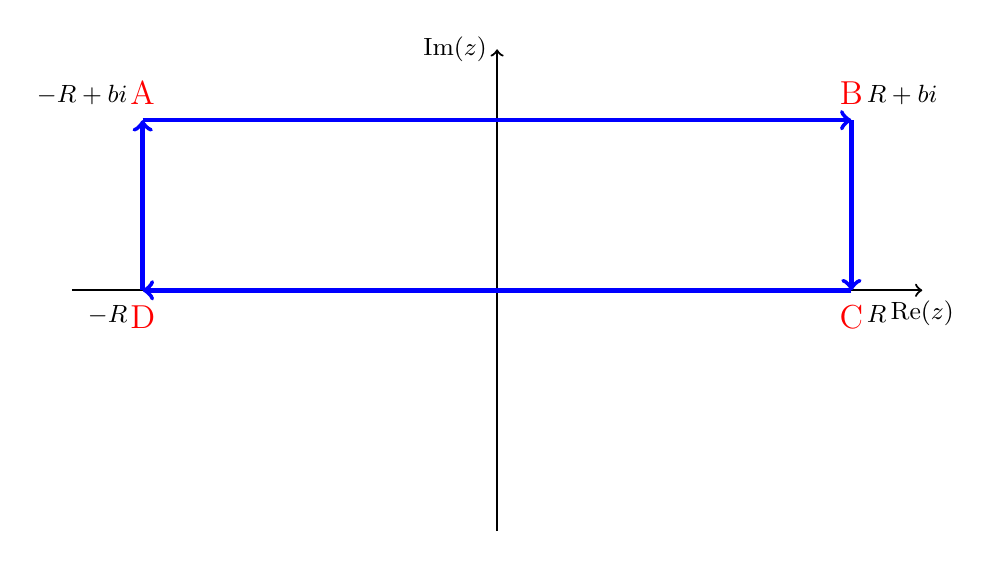
\begin{tikzpicture}[scale=1.8, font=\small]
				% Define coordinates
				\def\R{2.5}
				\def\b{1.2}
				
				% Draw axes
				\draw[->, thick] (-\R-0.5, 0) -- (\R+0.5, 0) node[below] {$\mathrm{Re}(z)$};
				% Adjusted y-axis to not overlap with labels
				\draw[->, thick] (0, -\b-0.5) -- (0, \b+0.5) node[left] {$\mathrm{Im}(z)$};
				
				% Define the vertex coordinates
				\coordinate (D) at (-\R, 0);
				\coordinate (C) at (\R, 0);
				\coordinate (B) at (\R, \b);
				\coordinate (A) at (-\R, \b);
				
				% --- MODIFICATION: Path labels C1, C2 etc. are removed ---
				% Draw paths with arrows only
				\draw[blue, ultra thick, ->] (C) -- (D);
				\draw[blue, ultra thick, ->] (B) -- (C);
				\draw[blue, ultra thick, ->] (A) -- (B);
				\draw[blue, ultra thick, ->] (D) -- (A);
				
				% Add vertex coordinate labels (black)
				\node[below left=2pt] at (D) {$-R$};
				\node[below right=2pt] at (C) {$R$};
				\node[above right=2pt] at (B) {$R+bi$};
				\node[above left=2pt] at (A) {$-R+bi$};
				
				% Add vertex letter labels (red), positioned to avoid overlap
				\node[red, above=2pt, font=\large] at (A) {A};
				\node[red, above=2pt, font=\large] at (B) {B};
				\node[red, below=2pt, font=\large] at (C) {C};
				\node[red, below=2pt, font=\large] at (D) {D};
				
			\end{tikzpicture}
		\end{center}
		
		根据柯西积分定理,函数在闭合围道上的积分为零:
		\begin{equation}\label{kexi}
			\oint_C e^{-az^2} dz = \int_{AB} e^{-az^2} dz + \int_{BC} e^{-az^2} dz + \int_{CD} e^{-az^2} dz + \int_{DA} e^{-az^2} dz = 0
		\end{equation}
		
		我们分别计算 $R \to \infty$ 时各段路径的积分。
		
		
		
		\textbf{1. 路径 $BC$ 与 $DA$:}
		在路径 $BC$ 上,参数化为 $z = R+iy$, $z(b) = R+ib$,$z(0) = R$,$dz=idy$, 其中 $y$ 从 $0$ 到 $b$。
		\begin{equation*}
			\left| \int_{BC} e^{-az^2} dz \right|= \left| \int_{R+bi}^{R} e^{-a(R+iy)^2} i dy \right|= \left| \int_{b}^{0} e^{-a(R+iy)^2} i dy \right| \le \int_{b}^{0} |e^{-a(R^2 - y^2 + 2iRy)}| dy 
		\end{equation*}
		\begin{equation*}
			= \int_{b}^{0} e^{-aR^2} e^{ay^2} dy = e^{-aR^2} \int_{b}^{0} e^{ay^2} dy
		\end{equation*}
		由于 $\int_{b}^{0} e^{ay^2} dy$ 是一个关于 $b$ 的常数,而 $\lim_{R \to \infty} e^{-aR^2} = 0$,所以:
		\begin{equation*}
			\lim_{R \to \infty} \left| \int_{BC} e^{-az^2} dz \right| = 0
		\end{equation*}
		同理可证,路径 $AD$ 的积分也为零。
		
		\textbf{2. 路径 $AB$:}
		在路径 $AB$ 上,参数化为 $z=x+bi$, $dz=dx$, 其中 $x$ 从 $R$ 变化到 $-R$。,由柯西积分公式\eqref{kexi}可知
		\begin{equation*}
			\int_{BA} e^{-az^2} dz = -	\int_{CD} e^{-az^2} dz = \int_{DC}e^{-az^2} dz= 	\lim_{R \to \infty}\int_{-R}^{R}e^{-ax^2} dx=\sqrt{\frac{\pi}{a}}
		\end{equation*}
		
		
		这证明了高斯积分的结果可以从实变量推广到复变量。
		
	\end{proof}
	
	
	
	
	\begin{proposition}\label{ex:3}
		$\int_{-\infty}^{+\infty} \cos kx \cdot e^{-a x^2} dx=\int_{-\infty}^{+\infty} e^{ikx} \cdot e^{-a x^2} dx= e^{-\frac{k^2}{4a}} \cdot \sqrt{\frac{\pi}{a}}$
	\end{proposition}
	
	\begin{proof}
		
		\begin{equation*}
			\int_{-\infty}^{+\infty} e^{ikx} \cdot e^{-a x^2} dx =\int_{-\infty}^{+\infty} \cos kx \cdot e^{-a x^2} dx+i\int_{-\infty}^{+\infty} \sin kx \cdot e^{-a x^2} dx
		\end{equation*}
		第二项为奇函数,积分为0,所以,
		\begin{equation*}
			\int_{-\infty}^{+\infty} e^{ikx} \cdot e^{-a x^2} dx =\int_{-\infty}^{+\infty} \cos kx \cdot e^{-a x^2} dx
		\end{equation*}
		
		\begin{equation*}
			\int_{-\infty}^{+\infty} e^{ikx} \cdot e^{-a x^2} dx = \int_{-\infty}^{+\infty} e^{-a x^2 + ikx} dx
		\end{equation*}
		
		配方
		\begin{equation*}
			\begin{split}
				-a x^2 + ikx &= -a \left( x^2 - \frac{ik}{a} x \right) \\
				&= -a \left[ x^2 - \frac{ik}{a} x + \left( \frac{ik}{2a} \right)^2 - \left( \frac{ik}{2a} \right)^2 \right] \\
				&= -a \left( x - \frac{ik}{2a} \right)^2 - \frac{k^2}{4a}
			\end{split}
		\end{equation*}
		所以,
		\begin{equation*}
			\int_{-\infty}^{+\infty} e^{ikx} \cdot e^{-a x^2} dx = \int_{-\infty}^{+\infty} e^{-a x^2 + ikx} dx	= e^{-\frac{k^2}{4a}} \cdot \sqrt{\frac{\pi}{a}}
		\end{equation*}
	\end{proof}
	
	\begin{corollary}
		我们计算高斯函数 $f(x) = e^{-ax^2}$ 的傅里叶变换。
		\begin{align*}
			\mathcal{F}\{f\}(w) &= \frac{1}{\sqrt{2\pi}} \int_{-\infty}^{+\infty} e^{-ax^2} e^{-iwx} dx \\
			&= \frac{1}{\sqrt{2\pi}} \int_{-\infty}^{+\infty} e^{-(ax^2 + iwx)} dx
		\end{align*}
	\end{corollary}
	
	
	为了计算这个积分,我们对指数部分进行配方:
	\begin{align*}
		ax^2 + iwx &= a\left(x^2 + \frac{iw}{a}x\right) \\
		&= a\left[ x^2 + 2 \cdot x \cdot \frac{iw}{2a} + \left(\frac{iw}{2a}\right)^2 - \left(\frac{iw}{2a}\right)^2 \right] \\
		&= a\left[ \left(x + \frac{iw}{2a}\right)^2 - \frac{i^2w^2}{4a^2} \right] \\
		&= a\left(x + \frac{iw}{2a}\right)^2 + a\left(\frac{w^2}{4a^2}\right) \\
		&= a\left(x + \frac{iw}{2a}\right)^2 + \frac{w^2}{4a}
	\end{align*}
	
	将配方后的结果代回积分中:
	\begin{align*}
		\mathcal{F}\{f\}(w) &= \frac{1}{\sqrt{2\pi}} \int_{-\infty}^{+\infty} e^{ - \left[ a\left(x + \frac{iw}{2a}\right)^2 + \frac{w^2}{4a} \right] } dx \\
		&= \frac{1}{\sqrt{2\pi}} \int_{-\infty}^{+\infty} e^{-a\left(x + \frac{iw}{2a}\right)^2} e^{-\frac{w^2}{4a}} dx \\
		&= \frac{1}{\sqrt{2\pi}} e^{-\frac{w^2}{4a}} \int_{-\infty}^{+\infty} e^{-a\left(x + \frac{iw}{2a}\right)^2} dx
	\end{align*}
	
	根据命题\eqref{ex:2}:
	\begin{equation*}
		\int_{-\infty}^{+\infty} e^{-a\left(x + \frac{iw}{2a}\right)^2} dx  = \sqrt{\frac{\pi}{a}}
	\end{equation*}
	
	因此,最终结果为:
	\begin{align*}
		\mathcal{F}\{f\}(w) &= \frac{1}{\sqrt{2\pi}} e^{-\frac{w^2}{4a}} \cdot \sqrt{\frac{\pi}{a}} \\
		&= \frac{1}{\sqrt{2a}} e^{-\frac{w^2}{4a}}
	\end{align*}
	
	
	
	
	\begin{proposition}\label{ex:4}
		$\int_{-\infty}^{+\infty} z^2 e^{-a z^2} dz = \frac{1}{2} \pi^{\frac{1}{2}} a^{-\frac{3}{2}}$
	\end{proposition}
	
	\begin{proof}
		
		
		\begin{equation*}
			\text{设} \quad \Phi(a) = \int_{-\infty}^{+\infty} e^{-a z^2} dz = \sqrt{\frac{\pi}{a}}
		\end{equation*}
		
		\begin{equation*}
			\frac{d\Phi}{da} = -\int_{-\infty}^{+\infty} z^2 e^{-a z^2} dz = \frac{d}{da} \left( \pi^{\frac{1}{2}} a^{-\frac{1}{2}} \right) = \pi^{\frac{1}{2}} a^{-\frac{3}{2}} \cdot \left( -\frac{1}{2} \right)
		\end{equation*}
		
		\begin{equation*}
			\therefore \int_{-\infty}^{+\infty} z^2 e^{-a z^2} dz = \frac{1}{2} \pi^{\frac{1}{2}} a^{-\frac{3}{2}}
		\end{equation*}
	\end{proof}
	
	
	
	\begin{proposition}\label{ex:5}
		$	\int_{-\infty}^{+\infty} (z + bx)^2 e^{-a z^2} dz=	= \frac{1}{2} \pi^{\frac{1}{2}} a^{-\frac{3}{2}} + b^2 x^2 \sqrt{\frac{\pi}{a}}$
	\end{proposition}
	
	\begin{proof}
		展开得
		\begin{equation*}
			= \int_{-\infty}^{+\infty} z^2 e^{-a z^2} dz + \int_{-\infty}^{+\infty} 2 z b x e^{-a z^2} dz + b^2 x^2 \int_{-\infty}^{+\infty} e^{-a z^2} dz
		\end{equation*}
		
		\begin{equation*}
			= \frac{1}{2} \pi^{\frac{1}{2}} a^{-\frac{3}{2}} + b^2 x^2 \sqrt{\frac{\pi}{a}}
		\end{equation*}
		
	\end{proof}
	
	
	
	
	
	
	
	
	\subsection{解的导出}
	对于无界的热传导方程\eqref{wujierechuandao}:
	\begin{equation}
		\begin{cases}
			u_t - a\Delta u = 0, \\
			u(x, 0) = \varphi(x),
		\end{cases}
	\end{equation}
	
	设初值问题的解 \( u(x, t) \) 和初始数据 \( \varphi(x) \) 都可关于变量 \( x \) 进行 Fourier 变换,并记:
	\begin{equation}
		\hat{u}(\xi, t) = \int_{\mathbb{R}^n} u(x, t) e^{-i x \cdot \xi} dx,
	\end{equation}
	\begin{equation}
		\hat{\varphi}(\xi) = \int_{\mathbb{R}^n} \varphi(x) e^{-i x \cdot \xi} dx.
	\end{equation}
	
	对热传导方程和初始条件进行 Fourier 变换,根据傅里叶的微分性质\eqref{weifen}:
	\begin{equation}
		\hat{u_t}=\int_{\mathbb{R}^n} u_t(x, t) e^{-i x \cdot \xi} dx=\frac{d}{dt} \int_{\mathbb{R}^n} u(x, t) e^{-i x \cdot \xi} dx= \frac{d\hat{u}(\xi, t)}{dt}
	\end{equation}
	
	\[
	\Delta u = \sum_{j=1}^n \frac{\partial^2 u}{\partial x_j^2}
	\]
	\[
	\mathcal{F}\left[\frac{\partial^2 u}{\partial x_j^2}\right](\xi) = -\xi_j^2 \hat{u}(\xi)
	\]
	\begin{equation}
		\mathcal{F}[\Delta u](\xi) = \sum_{j=1}^n (-\xi_j^2) \hat{u}(\xi) = -|\xi|^2 \hat{u}(\xi)
	\end{equation}
	
	
	把$\xi$看作常量,得到关于 \(\hat{u}(\xi, t)\) 的常微分方程初值问题:
	\begin{equation}
		\begin{cases}
			\displaystyle \frac{d\hat{u}(\xi, t)}{dt} + a|\xi|^2 \hat{u}(\xi, t) = 0, \\
			\hat{u}(\xi, 0) = \hat{\varphi}(\xi).
		\end{cases}
	\end{equation}
	该方程的解为:
	\begin{equation}
		\hat{u}(\xi, t) = \hat{\varphi}(\xi) e^{-a|\xi|^2 t}.
	\end{equation}
	
	
	
	\begin{proof}
		这是一个一阶线性常微分方程,可以通过分离变量法求解。
		将方程改写为:
		\[
		\frac{d\hat{u}}{\hat{u}} = -a |\xi|^2 dt
		\]
		
		对两边积分:
		\[
		\int \frac{d\hat{u}}{\hat{u}} = \int -a |\xi|^2 dt
		\]
		
		得到:
		\[
		\ln|\hat{u}| = -a |\xi|^2 t + C(\xi)
		\]
		其中,\(C(\xi)\) 是积分常数,可能依赖于 \(\xi\)。
		
		
		利用初始条件 \(\hat{u}(\xi, 0) = \hat{\varphi}(\xi)\),代入上式得:
		\[
		C(\xi) = \ln|\hat{\varphi}(\xi)|
		\]
		
		将 \(C(\xi)\) 代入积分结果:
		\[
		\ln|\hat{u}| = -a |\xi|^2 t + \ln|\hat{\varphi}(\xi)|
		\]
		
		对两边取指数:
		\[
		\hat{u}(\xi, t) = \hat{\varphi}(\xi) e^{-a |\xi|^2 t}
		\]
		
		
	\end{proof}
	
	
	对 \(\hat{u}(\xi, t)\) 进行 Fourier 逆变换
	\begin{equation}
		u(x, t) = \mathcal{F}^{-1}[\hat{\varphi}(\xi) e^{-a|\xi|^2 t}]
	\end{equation}
	
	利用Fourier 逆变换卷积的性质\eqref{nibianhuanjuanji}:
	\begin{equation}
		u(x, t) = \mathcal{F}^{-1}[\hat{\varphi}(\xi)] * \mathcal{F}^{-1}[e^{-a|\xi|^2 t}]
	\end{equation}
	
	\begin{proposition}
		我们需要证明:
		\[
		\mathcal{F}^{-1}\left[e^{-a|\xi|^2 t}\right](x) = (4\pi a t)^{-n/2} e^{-\frac{|x|^2}{4a t}}
		\]
	\end{proposition}
	
	
	
	\begin{proof}
		
		根据傅里叶逆变换的定义:
		\[
		\mathcal{F}^{-1}\left[e^{-a|\xi|^2 t}\right](x) = \frac{1}{(2\pi)^n} \int_{\mathbb{R}^n} e^{i x \cdot \xi} e^{-a|\xi|^2 t} d\xi
		\]
		
		我们可以将这个积分分解为每个坐标的积分:
		\[
		\mathcal{F}^{-1}\left[e^{-a|\xi|^2 t}\right](x) = \frac{1}{(2\pi)^n} \prod_{j=1}^n \int_{-\infty}^\infty e^{i x_j \xi_j} e^{-a\xi_j^2 t} d\xi_j
		\]
		
		\begin{remark}
			\[
			\mathcal{F}^{-1}\left[e^{-a|\xi|^{2} t}\right](x)=\frac{1}{(2\pi)^{n}}\prod_{j=1}^{n}\left(\int_{-\infty}^{\infty} e^{i x_j \xi_j} e^{-a\xi_j^{2} t} d\xi_j\right)
			\]
		\end{remark}
		
		
		对于每个一维积分,我们有:
		\[
		\int_{-\infty}^\infty e^{i x_j \xi_j} e^{-a\xi_j^2 t} d\xi_j
		\]
		
		对指数部分进行配方:
		\[
		-a t \xi_j^2 + i x_j \xi_j = -a t \left( \xi_j^2 - \frac{i x_j}{a t} \xi_j \right)
		\]
		\[
		= -a t \left( \xi_j^2 - \frac{i x_j}{a t} \xi_j + \left( \frac{x_j}{2a t} \right)^2 - \left( \frac{x_j}{2a t} \right)^2 \right)
		\]
		\[
		= -a t \left( \left( \xi_j - \frac{i x_j}{2a t} \right)^2 - \frac{x_j^2}{4a^2 t^2} \right)
		\]
		\[
		= -a t \left( \xi_j - \frac{i x_j}{2a t} \right)^2 + \frac{x_j^2}{4a t}
		\]
		
		代入积分中,由命题\eqref{ex:1}:
		\[
		\int_{-\infty}^\infty e^{-a t \left( \xi_j - \frac{i x_j}{2a t} \right)^2 + \frac{x_j^2}{4a t}} d\xi_j = e^{\frac{x_j^2}{4a t}} \int_{-\infty}^\infty e^{-a t \left( \xi_j - \frac{i x_j}{2a t} \right)^2} d\xi_j= \sqrt{\frac{\pi}{a t}} e^{\frac{x_j^2}{4a t}}
		\]
		
		
		将所有坐标的结果相乘,并乘以系数 \( \frac{1}{(2\pi)^n} \),得到:
		\[
		\mathcal{F}^{-1}\left[e^{-a|\xi|^2 t}\right](x) = \frac{1}{(2\pi)^n} \left( \sqrt{\frac{\pi}{a t}} \right)^n e^{-\frac{|x|^2}{4a t}}
		\]
		\[
		= \frac{1}{(2\pi)^n} \cdot \frac{\pi^{n/2}}{(a t)^{n/2}} e^{-\frac{|x|^2}{4a t}} = (4\pi a t)^{-n/2} e^{-\frac{|x|^2}{4a t}}
		\]
		
	\end{proof}
	
	
	
	
	
	因此,解可以表示为:
	\begin{equation}
		u(x, t) = \frac{1}{(4\pi a t)^{n/2}} \int_{\mathbb{R}^n} \varphi(y) e^{-\frac{|x - y|^2}{4a t}} dy
	\end{equation}
	相关例题可以去看第三次作业的最后一题\href{https://github.com/Albert-Chen04/Partial-differential-equation}{偏微分第三次作业}
	
		\newpage
	\section{无界非齐次热传导方程}
	和之前波动方程齐次化一样,先用叠加原理分解成两个子问题,用Duhamamel原理把方程齐次化。
	
	对于无界基础方程,把基本解看作达朗贝尔公式。
	
	\section{半直线热传导方程}
	把无界基础方程的基本解(泊松公式)看作达朗贝尔公式,第一边界用奇延拓,第二边界用偶延拓。
	
	
	\section{有界非齐次热传导方程}
	先用叠加原理分解成三个子问题,用Duhamamel原理把方程齐次化,用插值边界齐次化。
	
	对于有界基本方程用分离变量法,过程和波动的一样,就是时间常微分函数变成一阶通解为指数函数,而不再是三角函数。系数由边界条件决定,其他全部的求解过程,验证过程全部一样。
	
	也可以像达朗贝尔公式那样,满足相容性条件做奇偶延拓,再做周期延拓。
	可以参考下面这篇文章
\href{https://kns.cnki.net/kcms2/article/abstract?v=VQ0ntgfwFMTzN6hnFDpFMFM9DxAtYwMQhco2QSA-IEHGx9q5EylUyfVfvJ65vLbYgxi4GKWYtrw0WYFjulce4L-QdEJiwrbko6gMtLg1u_v-yZO9l1KqPNK5VVy0WXMK_iyRkdOb_3JYM79j78dC5ZO49R0B00eT_N_tEe4_tT88MKGKuKknjw==&uniplatform=NZKPT&language=CHS}{偏微分方程课程研究型教学的一个实例剖析,朱长江}
		\newpage
	\section{二阶线性偏微分方程按特征分类与标准化}
	\subsection{二阶方程的特征理论}
	考虑两个自变量的二阶拟线性偏微分方程的一般形式:
	\begin{equation}\label{eq:quasi_linear_2nd_order}
		a u_{xx} + b u_{xy} + c u_{yy} = F,
	\end{equation}
	其中系数 \(a, b, c\) 和非齐次项 \(F\) 都是 \(x, y, u, u_x, u_y\) 的已知函数。
	
	假设 \(\Gamma\) 是平面 \(xoy\) 上的一条光滑曲线,我们在这条曲线上给定所谓的 柯西初值条件 ,即函数 \(u\) 及其一阶偏导数的值:
	\begin{equation}\label{eq:cauchy_conditions_general}
		u|_{\Gamma} = \text{已知}, \quad u_x|_{\Gamma} = \text{已知}, \quad u_y|_{\Gamma} = \text{已知}.
	\end{equation}
	这样的定解问题称为 柯西问题 。核心问题是:定解问题 \eqref{eq:quasi_linear_2nd_order} 和 \eqref{eq:cauchy_conditions_general} 的解是否存在且唯一?
	
	为了回答这个问题,我们退一步思考:能否根据给定的方程和初值条件,唯一地确定解的所有二阶偏导数 \(u_{xx}, u_{xy}, u_{yy}\) 在曲线 \(\Gamma\) 上的值?如果连二阶导数都无法确定,解的存在唯一性就无从谈起。
	
	设曲线 \(\Gamma\) 的参数方程为 \(x = \varphi(s), y = \psi(s)\)。那么,柯西条件 \eqref{eq:cauchy_conditions_general} 可以更具体地写为:
	\begin{equation}\label{eq:cauchy_conditions_parametric}
		\begin{cases}
			u|_{\Gamma} = u(\varphi(s), \psi(s)) = u^0(s), \\
			u_x|_{\Gamma} = u_x(\varphi(s), \psi(s)) = p^0(s), \\
			u_y|_{\Gamma} = u_y(\varphi(s), \psi(s)) = q^0(s),
		\end{cases}
	\end{equation}
	其中 \(u^0(s), p^0(s), q^0(s)\) 是已知的函数。
	
	首先,这三个给定的函数并非完全独立。对 \eqref{eq:cauchy_conditions_parametric} 中第一个式子沿曲线 \(\Gamma\) 对参数 \(s\) 求导,根据链式法则有:
	\[
	\frac{\diff u^0(s)}{\diff s} = \frac{\partial u}{\partial x} \frac{\diff x}{\diff s} + \frac{\partial u}{\partial y} \frac{\diff y}{\diff s} = u_x \varphi'(s) + u_y \psi'(s).
	\]
	将 \(u_x\) 和 \(u_y\) 在 \(\Gamma\) 上的值代入,我们得到如下的相容性条件 :
	\begin{equation}
		(u^0(s))' = p^0(s)\varphi'(s) + q^0(s)\psi'(s).
	\end{equation}
	这表明初始数据必须满足此条件。
	
	接下来,为了求出二阶导数,我们自然地想到对 \eqref{eq:cauchy_conditions_parametric} 中的后两个式子也沿 \(\Gamma\) 对 \(s\) 求导:
	\begin{align}
		(p^0(s))' = \frac{\diff u_x}{\diff s} &= u_{xx}\varphi'(s) + u_{xy}\psi'(s), \label{eq:deriv_eq1} \\
		(q^0(s))' = \frac{\diff u_y}{\diff s} &= u_{yx}\varphi'(s) + u_{yy}\psi'(s). \label{eq:deriv_eq2}
	\end{align}
	假设解 \(u\) 是二次连续可微的,即 \(u_{xy} = u_{yx}\)。现在,我们将方程 \eqref{eq:quasi_linear_2nd_order} 本身(在曲线 \(\Gamma\) 上成立)与上面两个求导得到的式子 \eqref{eq:deriv_eq1}、\eqref{eq:deriv_eq2} 联立,得到一个关于三个未知量 \(u_{xx}, u_{xy}, u_{yy}\) 的线性方程组:
	\begin{equation}
		\begin{cases}
			a u_{xx} + b u_{xy} + c u_{yy} = F, \\
			\varphi'(s) u_{xx} + \psi'(s) u_{xy} = (p^0(s))', \\
			\varphi'(s) u_{xy} + \psi'(s) u_{yy} = (q^0(s))'.
		\end{cases}
	\end{equation}
	这个线性系统的系数行列式 \(D\) 为:
	\begin{equation}
		D = 
		\begin{vmatrix}
			a & b & c \\
			\varphi' & \psi' & 0 \\
			0 & \varphi' & \psi'
		\end{vmatrix}
		= a(\psi')^2 - b\varphi'\psi' + c(\varphi')^2.
	\end{equation}
	
	\begin{definition}[特征曲线]
		\begin{enumerate}[label=(\roman*)]
			\item 如果行列式 \(D \neq 0\),则线性方程组有唯一解。这意味着我们可以在曲线 \(\Gamma\) 上唯一地确定所有二阶偏导数的值。这样的曲线 \(\Gamma\) 称为方程 \eqref{eq:quasi_linear_2nd_order} 的非特征曲线。
			\item 如果行列式 \(D = 0\),则线性方程组的解不是唯一的(可能有无穷多解或无解,取决于右侧的常数项)。这意味着我们无法在 \(\Gamma\) 上唯一确定二阶导数。这样的曲线 \(\Gamma\) 称为方程 \eqref{eq:quasi_linear_2nd_order} 的特征曲线 。
		\end{enumerate}
	\end{definition}
	
	特征曲线满足的方程 \(D=0\) 称为特征方程 :
	\begin{equation}\label{eq:characteristic_eq_parametric}
		a(\psi'(s))^2 - b\varphi'(s)\psi'(s) + c(\varphi'(s))^2 = 0.
	\end{equation}
	注意到 \(\varphi'(s) = \frac{\diff x}{\diff s}\) 且 \(\psi'(s) = \frac{\diff y}{\diff s}\)。用 \((\diff s)^2\) 除以上式,并考虑到在特征曲线上 \(\frac{\diff y}{\diff x} = \frac{\psi'(s)}{\varphi'(s)}\),我们得到特征方程的微分形式:
	\begin{equation}\label{eq:characteristic_ode}
		a \left(\frac{\diff y}{\diff x}\right)^2 - b \frac{\diff y}{\diff x} + c = 0.
	\end{equation}
	这是一个关于 \(\frac{\diff y}{\diff x}\) 的二次方程,解出它就得到了特征曲线的斜率。
	
	
	\subsection{方程的分类与标准型}
	二阶线性方程的分类是基于特征方程的性质,这在可逆的自变量变换下是不变的。我们主要根据判别式 \(\Delta = b^2 - 4ac\) 的符号来分类。
	\begin{definition}[方程的分类]
		对于方程 \eqref{eq:quasi_linear_2nd_order}(这里我们考虑系数 \(a,b,c\) 仅依赖于 \(x,y\) 的线性情况),在某一点 \((x,y)\) 定义其判别式为 \(\Delta = b^2 - 4ac\)。
		\begin{itemize}
			\item 若 \(\Delta(x,y) > 0\),称方程在该点是双曲型 。
			\item 若 \(\Delta(x,y) = 0\),称方程在该点是抛物型 。
			\item 若 \(\Delta(x,y) < 0\),称方程在该点是椭圆型。
		\end{itemize}
	\end{definition}
	通过选择恰当的自变量变换,可以将方程化为最简形式,即标准型。这个变换的关键是利用特征曲线作为新的坐标线。
	
	\subsubsection{双曲型方程 (\texorpdfstring{$\Delta > 0$}{Delta > 0})}
	当 \(\Delta > 0\) 时,特征方程 \eqref{eq:characteristic_ode} 有两个不同的实数解,对应两族实特征曲线。
	\[
	\frac{\diff y}{\diff x} = \frac{b + \sqrt{b^2-4ac}}{2a} \quad \text{和} \quad \frac{\diff y}{\diff x} = \frac{b - \sqrt{b^2-4ac}}{2a}.
	\]
	积分这两组常微分方程,得到两族特征曲线 \(\varphi(x,y) = c_1\) 和 \(\psi(x,y) = c_2\)。
	我们选取新的坐标变换:
	\[
	\xi = \varphi(x,y), \quad \eta = \psi(x,y).
	\]
	在此变换下,可以证明新坐标系下的系数 \(A=0\) 且 \(C=0\),而 \(B \neq 0\)。原方程化为:
	\begin{equation}\label{eq:hyperbolic_canonical_1}
		u_{\xi\eta} + (\text{低阶项}) = 0.
	\end{equation}
	这称为双曲型方程的第一标准型。如果再做一个线性变换 \(\tilde{x} = \xi+\eta, \tilde{y}=\xi-\eta\),则可以消去混合偏导项,得到:
	\begin{equation}\label{eq:hyperbolic_canonical_2}
		u_{\tilde{x}\tilde{x}} - u_{\tilde{y}\tilde{y}} + (\text{低阶项}) = 0.
	\end{equation}
	这称为双曲型方程的第二标准型,典型的例子就是波动方程。
	
	\begin{proof}[第一标准型变换验证]
		我们来验证,当选取特征曲线 \(\varphi(x,y)=c_1\) 和 \(\psi(x,y)=c_2\) 作为新坐标 \(\xi=\varphi(x,y)\) 和 \(\eta=\psi(x,y)\) 时,新方程的系数 \(A\) 和 \(C\) 确实为零。
		
		在新坐标系下,二阶偏导项的系数为:
		\begin{align*}
			A &= a\varphi_x^2 + b\varphi_x\varphi_y + c\varphi_y^2 \\
			B &= a\varphi_x\psi_x + \frac{b}{2}(\varphi_x\psi_y + \varphi_y\psi_x) + c\varphi_y\psi_y \\
			C &= a\psi_x^2 + b\psi_x\psi_y + c\psi_y^2
		\end{align*}
		
		由于 \(\varphi(x,y)=c_1\) 是一条特征曲线,它的梯度向量 \((\varphi_x, \varphi_y)\) 与曲线的切线方向 \((\diff x, \diff y)\) 正交,即 \(\varphi_x \diff x + \varphi_y \diff y = 0\),所以 \(\frac{\diff y}{\diff x} = -\frac{\varphi_x}{\varphi_y}\)。
		
		将此代入特征方程 \eqref{eq:characteristic_ode}:
		\[
		a \left(-\frac{\varphi_x}{\varphi_y}\right)^2 - b \left(-\frac{\varphi_x}{\varphi_y}\right) + c = 0
		\]
		两边同乘以 \(\varphi_y^2\)(假设 \(\varphi_y \neq 0\)),得到:
		\[
		a\varphi_x^2 + b\varphi_x\varphi_y + c\varphi_y^2 = 0.
		\]
		这正是新系数 \(A\) 的表达式。因此,\(A=0\)。
		
		同理,由于 \(\psi(x,y)=c_2\) 也是一条特征曲线,可证 \(C=0\)。
		
		对于系数 \(B\),由于 \(\varphi\) 和 \(\psi\) 来自两个不同的特征根,它们是线性无关的,可以证明 \(B \neq 0\)。因此,方程成功化为只含混合偏导数 \(u_{\xi\eta}\) 的第一标准型。
	\end{proof}
	
	\begin{proof}[第二标准型变换验证]
		我们从双曲型方程的第一标准型出发:
		\[
		u_{\xi\eta} + D_0 u_\xi + E_0 u_\eta + G_0 u = F_0.
		\]
		引入新的线性变换:
		\[
		\tilde{x} = \xi + \eta, \quad \tilde{y} = \xi - \eta.
		\]
		反过来,我们有 \(\xi = \frac{1}{2}(\tilde{x}+\tilde{y})\) 和 \(\eta = \frac{1}{2}(\tilde{x}-\tilde{y})\)。
		
		我们的目标是计算 \(u_{\xi\eta}\) 如何用新坐标 \((\tilde{x}, \tilde{y})\) 的偏导数来表示。首先,使用链式法则计算一阶导数:
		\begin{align*}
			u_\xi &= \frac{\partial u}{\partial \xi} = \frac{\partial u}{\partial \tilde{x}}\frac{\partial \tilde{x}}{\partial \xi} + \frac{\partial u}{\partial \tilde{y}}\frac{\partial \tilde{y}}{\partial \xi} = u_{\tilde{x}} \cdot 1 + u_{\tilde{y}} \cdot 1 = u_{\tilde{x}} + u_{\tilde{y}}, \\
			u_\eta &= \frac{\partial u}{\partial \eta} = \frac{\partial u}{\partial \tilde{x}}\frac{\partial \tilde{x}}{\partial \eta} + \frac{\partial u}{\partial \tilde{y}}\frac{\partial \tilde{y}}{\partial \eta} = u_{\tilde{x}} \cdot 1 + u_{\tilde{y}} \cdot (-1) = u_{\tilde{x}} - u_{\tilde{y}}.
		\end{align*}
		
		接下来,计算混合偏导数 \(u_{\xi\eta}\)。我们将算子 \(\frac{\partial}{\partial \eta}\) 作用于 \(u_\xi\):
		\begin{align*}
			u_{\xi\eta} = \frac{\partial}{\partial \eta}(u_\xi) &= \frac{\partial}{\partial \eta}(u_{\tilde{x}} + u_{\tilde{y}}) \\
			&= \frac{\partial (u_{\tilde{x}})}{\partial \eta} + \frac{\partial (u_{\tilde{y}})}{\partial \eta}.
		\end{align*}
		再次应用链式法则:
		\begin{align*}
			\frac{\partial (u_{\tilde{x}})}{\partial \eta} &= \frac{\partial (u_{\tilde{x}})}{\partial \tilde{x}}\frac{\partial \tilde{x}}{\partial \eta} + \frac{\partial (u_{\tilde{x}})}{\partial \tilde{y}}\frac{\partial \tilde{y}}{\partial \eta} = u_{\tilde{x}\tilde{x}} \cdot 1 + u_{\tilde{x}\tilde{y}} \cdot (-1) = u_{\tilde{x}\tilde{x}} - u_{\tilde{x}\tilde{y}}, \\
			\frac{\partial (u_{\tilde{y}})}{\partial \eta} &= \frac{\partial (u_{\tilde{y}})}{\partial \tilde{x}}\frac{\partial \tilde{x}}{\partial \eta} + \frac{\partial (u_{\tilde{y}})}{\partial \tilde{y}}\frac{\partial \tilde{y}}{\partial \eta} = u_{\tilde{y}\tilde{x}} \cdot 1 + u_{\tilde{y}\tilde{y}} \cdot (-1) = u_{\tilde{y}\tilde{x}} - u_{\tilde{y}\tilde{y}}.
		\end{align*}
		将这两部分加起来,并利用 \(u_{\tilde{x}\tilde{y}} = u_{\tilde{y}\tilde{x}}\),我们得到:
		\[
		u_{\xi\eta} = (u_{\tilde{x}\tilde{x}} - u_{\tilde{x}\tilde{y}}) + (u_{\tilde{y}\tilde{x}} - u_{\tilde{y}\tilde{y}}) = u_{\tilde{x}\tilde{x}} - u_{\tilde{y}\tilde{y}}.
		\]
		
		现在,将 \(u_{\xi\eta}\), \(u_\xi\), 和 \(u_\eta\) 的新表达式代回第一标准型方程:
		\[
		(u_{\tilde{x}\tilde{x}} - u_{\tilde{y}\tilde{y}}) + D_0(u_{\tilde{x}} + u_{\tilde{y}}) + E_0(u_{\tilde{x}} - u_{\tilde{y}}) + G_0 u = F_0.
		\]
		整理后得到:
		\[
		u_{\tilde{x}\tilde{x}} - u_{\tilde{y}\tilde{y}} + (D_0+E_0)u_{\tilde{x}} + (D_0-E_0)u_{\tilde{y}} + G_0 u = F_0.
		\]
		这是一个只包含 \(u_{\tilde{x}\tilde{x}}\) 和 \(u_{\tilde{y}\tilde{y}}\) 作为二阶项的形式,即双曲型方程的第二标准型。
	\end{proof}
	化为第二标准型就是我们的波动方程,由达朗贝尔公式可知,双曲线方程可以写成第二标准型后两条特征线变量的组合,而且特征线变量不会杂糅到一起。
		\[
	u(\xi, \eta) = F(\xi) + G(\eta)
	\]
	
	\begin{example}
		判断下列方程的类型,并化成标准型:
		\[ 3u_{xx} + 2u_{xy} - u_{yy} + u_x + u_y = 0. \]
	\end{example}
	\begin{solution}
		步骤1. 判断类型
		
		系数 $A=3, B=2, C=-1$。判别式 $\Delta = B^2 - 4AC = 2^2 - 4(3)(-1) = 4+12=16>0$。方程为双曲型。
		
	步骤2. 求解特征方程
		
		特征方程为 $A(\frac{dy}{dx})^2 - B\frac{dy}{dx} + C = 0 \implies 3(\frac{dy}{dx})^2 - 2\frac{dy}{dx} - 1 = 0$。
		分解得 $(3\frac{dy}{dx}+1)(\frac{dy}{dx}-1)=0$。
		特征方向为 $\lambda_1 = 1$ 和 $\lambda_2 = -1/3$。
		对应的特征线方程为 $y-x=C_1$ 和 $y+\frac{1}{3}x=C_2$ (或 $3y+x=C_2$)。
		
		步骤3. 进行坐标变换
		
		取新坐标 $\xi = y-x, \eta=3y+x$。计算偏导数:
		\begin{align*}
			u_x &= u_\xi \xi_x + u_\eta \eta_x = -u_\xi + u_\eta \\
			u_y &= u_\xi \xi_y + u_\eta \eta_y = u_\xi + 3u_\eta \\
			u_{xx} &= \frac{\partial}{\partial x}(-u_\xi + u_\eta) = -(-u_{\xi\xi} + u_{\xi\eta}) + (-u_{\eta\xi} + u_{\eta\eta}) = u_{\xi\xi} - 2u_{\xi\eta} + u_{\eta\eta} \\
			u_{xy} &= \frac{\partial}{\partial y}(-u_\xi + u_\eta) = -(u_{\xi\xi} + 3u_{\xi\eta}) + (u_{\eta\xi} + 3u_{\eta\eta}) = -u_{\xi\xi} - 2u_{\xi\eta} + 3u_{\eta\eta} \\
			u_{yy} &= \frac{\partial}{\partial y}(u_\xi + 3u_\eta) = (u_{\xi\xi} + 3u_{\xi\eta}) + 3(u_{\eta\xi} + 3u_{\eta\eta}) = u_{\xi\xi} + 6u_{\xi\eta} + 9u_{\eta\eta}
		\end{align*}
		
		步骤4. 代入原方程化简
		
		二阶项: $3u_{xx} + 2u_{xy} - u_{yy} = 3(u_{\xi\xi} - 2u_{\xi\eta} + u_{\eta\eta}) + 2(-u_{\xi\xi} - 2u_{\xi\eta} + 3u_{\eta\eta}) - (u_{\xi\xi} + 6u_{\xi\eta} + 9u_{\eta\eta}) = (3-2-1)u_{\xi\xi} + (-6-4-6)u_{\xi\eta} + (3+6-9)u_{\eta\eta} = -16u_{\xi\eta}$。
		
	一阶项: $u_x + u_y = (-u_\xi + u_\eta) + (u_\xi + 3u_\eta) = 4u_\eta$。
		
		合并得到 $-16u_{\xi\eta} + 4u_\eta = 0$。两边同除以 $-4$,得到标准型:
		\[ 4u_{\xi\eta} - u_\eta = 0 \]
	\end{solution}
	
	\subsubsection{抛物型方程 (\texorpdfstring{$\Delta = 0$}{Delta = 0})}
	当 \(\Delta = 0\) 时,特征方程只有一个重实根 \(\frac{\diff y}{\diff x} = \frac{b}{2a}\),对应一族实特征曲线 \(\varphi(x,y)=c_1\)。我们取
	\[
	\xi = \varphi(x,y), \quad \eta = \text{任一与}\ \xi\ \text{独立的函数 (如 } \eta=x \text{ 或 } \eta=y).
	\]
	在此变换下,可以证明 \(A=0\) 且 \(B=0\),但 \(C \neq 0\)。原方程化为:
	\begin{equation}\label{eq:parabolic_canonical}
		u_{\eta\eta} + (\text{低阶项}) = 0.
	\end{equation}
	这称为抛物型方程的标准型,典型的例子是热传导方程。
	
	\begin{proof}[变换验证]
		当 \(\Delta = 0\) 时,只有一族特征曲线 \(\varphi(x,y)=c_1\)。我们取 \(\xi = \varphi(x,y)\)。根据双曲型的证明,我们已经知道新系数 \(A = a\varphi_x^2 + b\varphi_x\varphi_y + c\varphi_y^2 = 0\)。
		
		现在我们来验证 \(B\) 也为零。新系数 \(B\) 的表达式为:
		\[
		B = a\varphi_x\eta_x + \frac{b}{2}(\varphi_x\eta_y + \varphi_y\eta_x) + c\varphi_y\eta_y.
		\]
		由于 \(\Delta = b^2 - 4ac = 0\),我们有 \(b = 2\sqrt{ac}\) (或 \(-2\sqrt{ac}\))。特征方程 \(a\lambda^2 - b\lambda + c = 0\) 的唯一解为 \(\lambda = \frac{b}{2a}\)。
		因此,特征曲线满足 \(\frac{\diff y}{\diff x} = -\frac{\varphi_x}{\varphi_y} = \frac{b}{2a}\)。这意味着 \(\varphi_x\) 和 \(\varphi_y\) 的比值是固定的:
		\[
		-2a\varphi_x = b\varphi_y.
		\]
		将 \(b\varphi_y\) 替换为 \(-2a\varphi_x\),并将 \(c\) 替换为 \(\frac{b^2}{4a}\),代入 \(B\) 的表达式中:
		\begin{align*}
			B &= a\varphi_x\eta_x + \frac{b}{2}\varphi_x\eta_y + \frac{b}{2}\varphi_y\eta_x + c\varphi_y\eta_y \\
			&= a\varphi_x\eta_x + \frac{b}{2}\varphi_x\eta_y + \frac{b}{2}\left(-\frac{2a}{b}\varphi_x\right)\eta_x + \frac{b^2}{4a}\left(-\frac{2a}{b}\varphi_x\right)\eta_y \\
			&= a\varphi_x\eta_x + \frac{b}{2}\varphi_x\eta_y - a\varphi_x\eta_x - \frac{b}{2}\varphi_x\eta_y \\
			&= 0.
		\end{align*}
		由于我们选取的 \(\eta\) 与 \(\xi\) 线性无关,可以保证 \(C \neq 0\)。因此,方程成功化为只含二阶导数 \(u_{\eta\eta}\) 的标准型。由此可见其实另一变量取什么都可以,因为我们只用了第一个变量就可以完成标准化,但是为了简便,我们一般取$x$或$y$.
	\end{proof}
	
	\subsubsection{椭圆型方程 (\texorpdfstring{$\Delta < 0$}{Delta < 0})}
	当 \(\Delta < 0\) 时,特征方程有两个互为共轭的复数解,对应两族复特征曲线 \(\varphi(x,y) = c_1\) 和 \(\psi(x,y) = c_2\),其中 \(\psi = \bar{\varphi}\)。我们可以取两条复特征线。但因为取复数的计算很大,我们还可以一个取其中一条复特征线的实部,一个取其中一条复特征线的虚部:
	\[
	\xi = \text{Re}(\varphi(x,y)) = \frac{\varphi+\psi}{2}, \quad \eta = \text{Im}(\varphi(x,y)) = \frac{\varphi-\psi}{2i}.
	\]
	在此变换下,可以证明 \(A=C\) 且 \(B=0\)。原方程化为:
	\begin{equation}\label{eq:elliptic_canonical}
		u_{\xi\xi} + u_{\eta\eta} + (\text{低阶项}) = 0.
	\end{equation}
	这称为椭圆型方程的标准型,典型的例子是拉普拉斯方程。
	
	\begin{proof}[变换验证]
		在椭圆型情况下,特征曲线 \(\varphi(x,y)=c_1\) 和 \(\psi(x,y)=c_2\) 是共轭复函数,即 \(\psi = \bar{\varphi}\)。
		设 \(\varphi = \alpha + i\beta\),则 \(\psi = \alpha - i\beta\),其中 \(\alpha(x,y)\) 和 \(\beta(x,y)\) 是实函数。
		我们的新坐标是 \(\xi = \alpha(x,y)\) 和 \(\eta = \beta(x,y)\)。
		
		根据双曲型的推导,我们知道 \(A_\text{complex} = a\varphi_x^2 + b\varphi_x\varphi_y + c\varphi_y^2 = 0\)。
		将 \(\varphi = \xi + i\eta\) 代入上式:
		\[
		a(\xi_x+i\eta_x)^2 + b(\xi_x+i\eta_x)(\xi_y+i\eta_y) + c(\xi_y+i\eta_y)^2 = 0.
		\]
		展开并分离实部和虚部。
		
		实部:
		\[
		a(\xi_x^2-\eta_x^2) + b(\xi_x\xi_y - \eta_x\eta_y) + c(\xi_y^2-\eta_y^2) = 0.
		\]
		这可以写成:
		\[
		(a\xi_x^2 + b\xi_x\xi_y + c\xi_y^2) - (a\eta_x^2 + b\eta_x\eta_y + c\eta_y^2) = 0.
		\]
		这正是新坐标系下的系数 \(A-C=0\),所以 \(A=C\)。
		
		虚部:
		\[
		2a\xi_x\eta_x + b(\xi_x\eta_y + \xi_y\eta_x) + 2c\xi_y\eta_y = 0.
		\]
		这正是新坐标系下混合导数项系数 \(B\) 的表达式。所以 \(B=0\)。
		
		因此,方程成功化为 \(A(u_{\xi\xi} + u_{\eta\eta}) + \dots = 0\),即拉普拉斯形式的标准型。
	\end{proof}
	
\begin{proof}[变换验证]
	在椭圆型情况下,特征方程 \eqref{eq:characteristic_ode} 的根是共轭复数。这意味着对应的两族特征曲线 \(\varphi(x,y)=c_1\) 和 \(\psi(x,y)=c_2\) 是共轭复函数。
	
	我们可以只取其中一族,例如 \(\varphi(x,y) = \text{const}\)。由于 \(\varphi\) 是一个复值函数,我们可以将其分解为实部和虚部:
	\[
	\varphi(x,y) = \xi(x,y) + i\eta(x,y),
	\]
	其中 \(\xi(x,y)\) 和 \(\eta(x,y)\) 是实值函数。我们选择这两个实函数作为新的坐标。
	
	因为 \(\varphi(x,y)\) 满足特征方程,所以我们有:
	\begin{equation}\label{eq:complex_char_eq_phi}
		a\varphi_x^2 + b\varphi_x\varphi_y + c\varphi_y^2 = 0.
	\end{equation}
	现在,我们将 \(\varphi_x = \xi_x + i\eta_x\) 和 \(\varphi_y = \xi_y + i\eta_y\) 代入这个复数方程中:
	\[
	a(\xi_x + i\eta_x)^2 + b(\xi_x + i\eta_x)(\xi_y + i\eta_y) + c(\xi_y + i\eta_y)^2 = 0.
	\]
	展开这个表达式:
	\[
	a(\xi_x^2 - \eta_x^2 + 2i\xi_x\eta_x) + b(\xi_x\xi_y - \eta_x\eta_y + i(\xi_x\eta_y + \xi_y\eta_x)) + c(\xi_y^2 - \eta_y^2 + 2i\xi_y\eta_y) = 0.
	\]
	一个复数等于零,意味着它的实部和虚部都必须为零。
	
令实部为零:
	\[
	[a\xi_x^2 + b\xi_x\xi_y + c\xi_y^2] - [a\eta_x^2 + b\eta_x\eta_y + c\eta_y^2] = 0.
	\]
	在新坐标系 \(\xi, \eta\) 下,二阶项系数 \(A\) 和 \(C\) 的定义是:
	\begin{align*}
		A &= a\xi_x^2 + b\xi_x\xi_y + c\xi_y^2, \\
		C &= a\eta_x^2 + b\eta_x\eta_y + c\eta_y^2.
	\end{align*}
	因此,实部为零的条件恰好说明了 \(A - C = 0\),即 \(A=C\)。
	
令虚部为零:
	\[
	2a\xi_x\eta_x + b(\xi_x\eta_y + \xi_y\eta_x) + 2c\xi_y\eta_y = 0.
	\]
	在新坐标系下,混合偏导项 \(u_{\xi\eta}\) 的系数 \(B_\text{new}\) 是:
	\[
	B_\text{new} = 2a\xi_x\eta_x + b(\xi_x\eta_y + \xi_y\eta_x) + 2c\xi_y\eta_y.
	\]
	因此,虚部为零的条件恰好说明了 \(B_\text{new} = 0\)。
	
	综上所述,通过选取一个复特征函数的实部和虚部作为新的坐标,我们成功地使得新方程的系数满足 \(A=C\) 且混合项系数为零。这样,方程就化为了 \(A(u_{\xi\xi} + u_{\eta\eta}) + (\text{低阶项}) = 0\),这正是椭圆型方程的标准型。
\end{proof}

	\begin{example}
		判断 Tricomi 方程 \(u_{yy} - y u_{xx} = 0\) 的类型并化为标准型。
	\end{example}
	\begin{solution}
		这里 \(a=-y, b=0, c=1\)。判别式为 \(\Delta = b^2-4ac = 0^2 - 4(-y)(1) = 4y\)。
		\begin{itemize}
			\item \textbf{情形1:当 \(y > 0\) 时},\(\Delta > 0\),方程为双曲型。
			特征方程为 \(-y (\frac{\diff y}{\diff x})^2 + 1 = 0\),即 \(\frac{\diff y}{\diff x} = \pm \frac{1}{\sqrt{y}}\)。
			积分得两族特征曲线:
			\[
			\int y^{1/2} \diff y = \int \pm \diff x \implies \frac{2}{3}y^{3/2} = \pm x + C.
			\]
			即 \( x - \frac{2}{3}y^{3/2} = c_1 \) 和 \( x + \frac{2}{3}y^{3/2} = c_2 \)。
			作变量代换:
			\[ \xi = x - \frac{2}{3}y^{3/2}, \quad \eta = x + \frac{2}{3}y^{3/2}. \]
			经过计算,可将方程化为第一标准型:
			\[ u_{\xi\eta} - \frac{1}{6(\eta-\xi)}(u_\eta - u_\xi) = 0. \]
			
			\item \textbf{情形2:当 \(y < 0\) 时},\(\Delta < 0\),方程为椭圆型。
			特征方程为 \(\frac{\diff y}{\diff x} = \pm \frac{i}{\sqrt{-y}}\)。
			积分得两族复特征曲线:
			\[
			\int (-y)^{1/2} \diff y = \int \pm i \diff x \implies -\frac{2}{3}(-y)^{3/2} = \pm ix + C.
			\]
			取实部和虚部作变量代换:
			\[ \xi = x, \quad \eta = \frac{2}{3}(-y)^{3/2}. \]
			经过计算,可将方程化为标准型:
			\[ u_{\xi\xi} + u_{\eta\eta} + \frac{1}{3\eta}u_\eta = 0. \]
			
			\item \textbf{情形3:当 \(y = 0\) 时},\(\Delta = 0\),方程为抛物型。这条线是类型的退化线。
		\end{itemize}
		Tricomi 方程是在不同区域呈现不同类型的混合型方程的典型例子。
	\end{solution}
	
	\newpage
	\section{多个自变量特征曲面与特征方程}
	现在我们将特征理论推广到 \(n\) 个自变量的二阶线性偏微分方程。其一般形式为:
	\begin{equation}\label{eq:pde_n_vars}
		\sum_{i,j=1}^{n} a_{ij}(x) \frac{\partial^2 u}{\partial x_i \partial x_j} + \sum_{i=1}^{n} b_i(x) \frac{\partial u}{\partial x_i} + c(x) u = f(x),
	\end{equation}
	其中 \(x=(x_1, \dots, x_n)\),且我们假设主部系数矩阵是对称的,即 \(a_{ij} = a_{ji}\)。
	
	柯西问题是在 \(n\) 维空间 \(\R^n\) 中的一个 \(n-1\) 维光滑超曲面 \(S\) 上给定初值。设 \(S\) 由方程 \(G(x_1, \dots, x_n) = 0\) 定义。柯西数据通常是给定 \(u\) 在 \(S\) 上的值以及它在 \(S\) 上的法向导数。这等价于给定 \(u\) 和它的所有一阶偏导数 \(\frac{\partial u}{\partial x_i}\) 在 \(S\) 上的值。
	\begin{equation}\label{eq:cauchy_n_vars}
		u|_{S} = \varphi_0(x), \quad \frac{\partial u}{\partial x_i}\bigg|_{S} = \varphi_i(x), \quad i=1, \dots, n.
	\end{equation}
	同样,我们的问题是:能否在曲面 \(S\) 上唯一地确定所有的二阶偏导数 \(\frac{\partial^2 u}{\partial x_i \partial x_j}\)?
	
	\paragraph{特殊情形:超平面}
	我们首先考虑一个特殊情况,即超曲面 \(S\) 是一个坐标超平面,例如 \(S: x_n = x_n^0\)。此时,定解条件变为在 \(x_n=x_n^0\) 上给定 \(u\) 和 \(\nabla u\)。
	由于 \(u\) 在超平面 \(x_n=x_n^0\) 上的值 \(u(x_1, \dots, x_{n-1}, x_n^0)\) 是已知的,我们可以直接求出它关于前 \(n-1\) 个变量的任意阶切向导数,例如 \(\frac{\partial u}{\partial x_i}\) 和 \(\frac{\partial^2 u}{\partial x_i \partial x_j}\) 对于 \(i,j < n\)。
	因此,在 \(S\) 上,唯一不确定的二阶导数是包含对 \(x_n\) 求导的项,特别是纯法向二阶导数 \(\frac{\partial^2 u}{\partial x_n^2}\)。
	
	我们将方程 \eqref{eq:pde_n_vars} 中与 \(\frac{\partial^2 u}{\partial x_n^2}\) 相关的项分离出来:
	\[
	a_{nn} \frac{\partial^2 u}{\partial x_n^2} + 2\sum_{i=1}^{n-1} a_{in} \frac{\partial^2 u}{\partial x_i \partial x_n} + \sum_{i,j=1}^{n-1} a_{ij} \frac{\partial^2 u}{\partial x_i \partial x_j} + (\text{低阶项}) = f.
	\]
	移项后得到:
	\[
	a_{nn} \frac{\partial^2 u}{\partial x_n^2} = f - (\text{低阶项}) - 2\sum_{i=1}^{n-1} a_{in} \frac{\partial^2 u}{\partial x_i \partial x_n} - \sum_{i,j=1}^{n-1} a_{ij} \frac{\partial^2 u}{\partial x_i \partial x_j}.
	\]
	上式右边的所有项在超平面 \(S\) 上都是已知的。因此,能否唯一确定 \(\frac{\partial^2 u}{\partial x_n^2}\) 的值,完全取决于其系数 \(a_{nn}\) 在 \(S\) 上是否为零。
	\begin{itemize}
		\item 若 \(a_{nn}|_S \neq 0\),则 \(\frac{\partial^2 u}{\partial x_n^2}\) 可以被唯一确定。
		\item 若 \(a_{nn}|_S = 0\),则无法唯一确定 \(\frac{\partial^2 u}{\partial x_n^2}\)。此时,只有当右端恰好也为零时,问题才可能有解(且有无穷多解),这需要满足一个额外的相容性条件。
	\end{itemize}
	
	\paragraph{一般情形:任意曲面}
	对于由 \(G(x)=0\) 定义的一般光滑曲面 \(S\),我们可以通过一个局部坐标变换(称为拉直变换)将其拉直为一个超平面。
	假设在曲面 \(S\) 上一点 \(P\),\(\nabla G \neq 0\),不妨设 \(\frac{\partial G}{\partial x_n} \neq 0\)。我们定义新坐标 \((\xi_1, \dots, \xi_n)\) 如下:
	\begin{equation}
		\begin{cases}
			\xi_i = x_i, & i=1, \dots, n-1, \\
			\xi_n = G(x_1, \dots, x_n).
		\end{cases}
	\end{equation}
	根据隐函数定理,这是一个可逆的局部坐标变换。在这个新坐标系下,原来的曲面 \(S\) 变成了超平面 \(\xi_n = 0\)。
	
	原方程 \eqref{eq:pde_n_vars} 在新坐标系下会变成一个新的方程:
	\[
	\sum_{i,j=1}^{n} A_{ij}(\xi) \frac{\partial^2 u}{\partial \xi_i \partial \xi_j} + \sum_{i=1}^{n} B_i(\xi) \frac{\partial u}{\partial \xi_i} + C(\xi) u = F(\xi).
	\]
	根据我们在超平面情形下的分析,新方程能否唯一求解二阶法向导数 \(\frac{\partial^2 u}{\partial \xi_n^2}\),取决于其系数 \(A_{nn}\) 在 \(\xi_n=0\) 上是否为零。
	
	通过繁琐但直接的链式法则计算,可以得到新旧系数之间的关系。特别是,系数 \(A_{nn}\) 的表达式为:
	\[
	A_{nn} = \sum_{i,j=1}^{n} a_{ij} \frac{\partial \xi_n}{\partial x_i} \frac{\partial \xi_n}{\partial x_j} = \sum_{i,j=1}^{n} a_{ij} \frac{\partial G}{\partial x_i} \frac{\partial G}{\partial x_j}.
	\]
	因此,曲面 \(S: G(x)=0\) 是否为特征曲面,取决于 \(A_{nn}\) 是否为零。
	
	\begin{definition}[特征曲面与特征方程]
		对于 \(n\) 维二阶线性方程 \eqref{eq:pde_n_vars}:
		\begin{enumerate}[label=(\roman*)]
			\item 曲面 \(S: G(x)=0\) 称为特征曲面 ,如果它满足下面的方程:
			\begin{equation}\label{eq:char_surface_n_dim}
				\sum_{i,j=1}^{n} a_{ij}(x) \frac{\partial G}{\partial x_i} \frac{\partial G}{\partial x_j} = 0, \quad \forall x \in S.
			\end{equation}
			这个方程称为特征方程。
			\item 在曲面 \(S\) 上,柯西问题是不适定的。
			\item 如果曲面 \(S\) 不满足特征方程,则称其为非特征曲面。
		\end{enumerate}
	\end{definition}
	
	\begin{remark}
		注意到向量 \((\frac{\partial G}{\partial x_1}, \dots, \frac{\partial G}{\partial x_n})\) 是曲面 \(G=0\) 的法向量。如果记该法向量的方向余弦为 \((\alpha_1, \dots, \alpha_n)\),那么特征方程也可以写成二次型的形式:
		\[
		\sum_{i,j=1}^{n} a_{ij} \alpha_i \alpha_j = 0.
		\]
		满足此方程的方向称为特征方向。特征曲面就是其上每一点的法向都是特征方向的曲面。
	\end{remark}
	
	
		\begin{example}
		写出方程 $u_{xy} + u_{yz} + u_{zz} = 0$ 的特征方程。
	\end{example}
	\begin{solution}
		设特征曲面为 $\phi(x, y, z) = C$。特征方程由主部系数决定,其形式为:
		\[
		\phi_x \phi_y + \phi_y \phi_z + \phi_z^2 = 0
		\]
	\end{solution}
	
	
	\begin{example}
		求 \(n\) 维 Laplace 方程 \(\Delta u = \sum_{i=1}^n u_{x_ix_i} = 0\) 的特征曲面。
	\end{example}
	\begin{solution}
		这里,主部系数 \(a_{ij} = \delta_{ij}\) (Kronecker delta),即 \(a_{ii}=1\),当 \(i \neq j\) 时 \(a_{ij}=0\)。
		特征方程为:
		\[
		\sum_{i,j=1}^{n} \delta_{ij} \frac{\partial G}{\partial x_i} \frac{\partial G}{\partial x_j} = \sum_{i=1}^{n} \left(\frac{\partial G}{\partial x_i}\right)^2 = |\nabla G|^2 = 0.
		\]
		对于实函数 \(G\),\(|\nabla G|^2=0\) 意味着 \(\nabla G = 0\),这与 \(G=0\) 定义了一个光滑曲面的前提(\(\nabla G \neq 0\))相矛盾。
		因此,Laplace 方程在实数域内没有任何特征曲面。这与椭圆型方程的性质是一致的,即任何曲面都是非特征的,可以在任意光滑边界上提出适定的定解问题(如 Dirichlet 或 Neumann 问题)。
	\end{solution}
	
	
	
	
	%弱解
%	\href{https://en.wikipedia.org/wiki/Weak_solution}{(Weak Solution)}
	
	%\newpage
	
\end{document}